\documentclass[final]{scrreprt} %scrreprt of scrartcl
% Include all project wide packages here.
\usepackage{fullpage}
\usepackage{polyglossia}
\setmainlanguage{english}
\usepackage{csquotes}
\usepackage{graphicx}
\usepackage{epstopdf}
\usepackage{pdfpages}
\usepackage{caption}
\usepackage[list=true]{subcaption}
\usepackage{float}
\usepackage{standalone}
\usepackage{import}
\usepackage{tocloft}
\usepackage{wrapfig}
\usepackage{authblk}
\usepackage{array}
\usepackage{booktabs}
\usepackage[toc,page,title,titletoc]{appendix}
\usepackage{xunicode}
\usepackage{fontspec}
\usepackage{pgfplots}
\usepackage{SIunits}
\usepackage{units}
\pgfplotsset{compat=newest}
\pgfplotsset{plot coordinates/math parser=false}
\newlength\figureheight 
\newlength\figurewidth
\usepackage{amsmath}
\usepackage{mathtools}
\usepackage{unicode-math}
\usepackage[
    backend=bibtexu,
	texencoding=utf8,
bibencoding=utf8,
    style=ieee,
    sortlocale=en_US,
    language=auto
]{biblatex}
\usepackage{listings}
\newcommand{\includecode}[3][c]{\lstinputlisting[caption=#2, escapechar=, style=#1]{#3}}
\newcommand{\superscript}[1]{\ensuremath{^{\textrm{#1}}}}
\newcommand{\subscript}[1]{\ensuremath{_{\textrm{#1}}}}


\newcommand{\chapternumber}{\thechapter}
\renewcommand{\appendixname}{Bijlage}
\renewcommand{\appendixtocname}{Bijlagen}
\renewcommand{\appendixpagename}{Bijlagen}

\usepackage[hidelinks]{hyperref} %<--------ALTIJD ALS LAATSTE

\renewcommand{\familydefault}{\sfdefault}

\setmainfont[Ligatures=TeX]{Myriad Pro}
\setmathfont{Asana Math}
\setmonofont{Lucida Console}

\usepackage{titlesec, blindtext, color}
\definecolor{gray75}{gray}{0.75}
\newcommand{\hsp}{\hspace{20pt}}
\titleformat{\chapter}[hang]{\Huge\bfseries}{\chapternumber\hsp\textcolor{gray75}{|}\hsp}{0pt}{\Huge\bfseries}
\renewcommand{\familydefault}{\sfdefault}
\renewcommand{\arraystretch}{1.2}
\setlength\parindent{0pt}

%For code listings
\definecolor{black}{rgb}{0,0,0}
\definecolor{browntags}{rgb}{0.65,0.1,0.1}
\definecolor{bluestrings}{rgb}{0,0,1}
\definecolor{graycomments}{rgb}{0.4,0.4,0.4}
\definecolor{redkeywords}{rgb}{1,0,0}
\definecolor{bluekeywords}{rgb}{0.13,0.13,0.8}
\definecolor{greencomments}{rgb}{0,0.5,0}
\definecolor{redstrings}{rgb}{0.9,0,0}
\definecolor{purpleidentifiers}{rgb}{0.01,0,0.01}


\lstdefinestyle{csharp}{
language=[Sharp]C,
showspaces=false,
showtabs=false,
breaklines=true,
showstringspaces=false,
breakatwhitespace=true,
escapeinside={(*@}{@*)},
columns=fullflexible,
commentstyle=\color{greencomments},
keywordstyle=\color{bluekeywords}\bfseries,
stringstyle=\color{redstrings},
identifierstyle=\color{purpleidentifiers},
basicstyle=\ttfamily\small}

\lstdefinestyle{c}{
language=C,
showspaces=false,
showtabs=false,
breaklines=true,
showstringspaces=false,
breakatwhitespace=true,
escapeinside={(*@}{@*)},
columns=fullflexible,
commentstyle=\color{greencomments},
keywordstyle=\color{bluekeywords}\bfseries,
stringstyle=\color{redstrings},
identifierstyle=\color{purpleidentifiers},
}

\lstdefinestyle{matlab}{
language=Matlab,
showspaces=false,
showtabs=false,
breaklines=true,
showstringspaces=false,
breakatwhitespace=true,
escapeinside={(*@}{@*)},
columns=fullflexible,
commentstyle=\color{greencomments},
keywordstyle=\color{bluekeywords}\bfseries,
stringstyle=\color{redstrings},
identifierstyle=\color{purpleidentifiers}
}

\lstdefinestyle{vhdl}{
language=VHDL,
showspaces=false,
showtabs=false,
breaklines=true,
showstringspaces=false,
breakatwhitespace=true,
escapeinside={(*@}{@*)},
columns=fullflexible,
commentstyle=\color{greencomments},
keywordstyle=\color{bluekeywords}\bfseries,
stringstyle=\color{redstrings},
identifierstyle=\color{purpleidentifiers}
}

\lstdefinestyle{xaml}{
language=XML,
showspaces=false,
showtabs=false,
breaklines=true,
showstringspaces=false,
breakatwhitespace=true,
escapeinside={(*@}{@*)},
columns=fullflexible,
commentstyle=\color{greencomments},
keywordstyle=\color{redkeywords},
stringstyle=\color{bluestrings},
tagstyle=\color{browntags},
morestring=[b]",
  morecomment=[s]{<?}{?>},
  morekeywords={xmlns,version,typex:AsyncRecords,x:Arguments,x:Boolean,x:Byte,x:Char,x:Class,x:ClassAttributes,x:ClassModifier,x:Code,x:ConnectionId,x:Decimal,x:Double,x:FactoryMethod,x:FieldModifier,x:Int16,x:Int32,x:Int64,x:Key,x:Members,x:Name,x:Object,x:Property,x:Shared,x:Single,x:String,x:Subclass,x:SynchronousMode,x:TimeSpan,x:TypeArguments,x:Uid,x:Uri,x:XData,Grid.Column,Grid.ColumnSpan,Click,ClipToBounds,Content,DropDownOpened,FontSize,Foreground,Header,Height,HorizontalAlignment,HorizontalContentAlignment,IsCancel,IsDefault,IsEnabled,IsSelected,Margin,MinHeight,MinWidth,Padding,SnapsToDevicePixels,Target,TextWrapping,Title,VerticalAlignment,VerticalContentAlignment,Width,WindowStartupLocation,Binding,Mode,OneWay,xmlns:x}
}

%defaults
\lstset{
basicstyle=\ttfamily\small,
extendedchars=false,
numbers=left,
numberstyle=\ttfamily\tiny,
stepnumber=1,
tabsize=4,
numbersep=5pt
}
\addbibresource{../library/bibliography.bib}
\title{Module 1 - Report}
\author{Alex {Misdorp} \and Xenia {Wesdijk}}
\begin{document}
\section{Task 1: Nissan Leaf}

As can be seen in fig \ref{fig:acceleration}, the Nissan Leaf will reach 96.6 km/h (60 mph) in just about nine seconds. Therefore the manufacturer's statement is true.
\\The limit on the motor's torque causes the vehicle to not accelerate any faster.
\\The small steady state error in the vehicle's velocity is caused by the driver's non-infinite gain in the simulation. Therefore, not enough motor torque is provided to reach the desired velocity.
\begin{figure}[H]
\centering
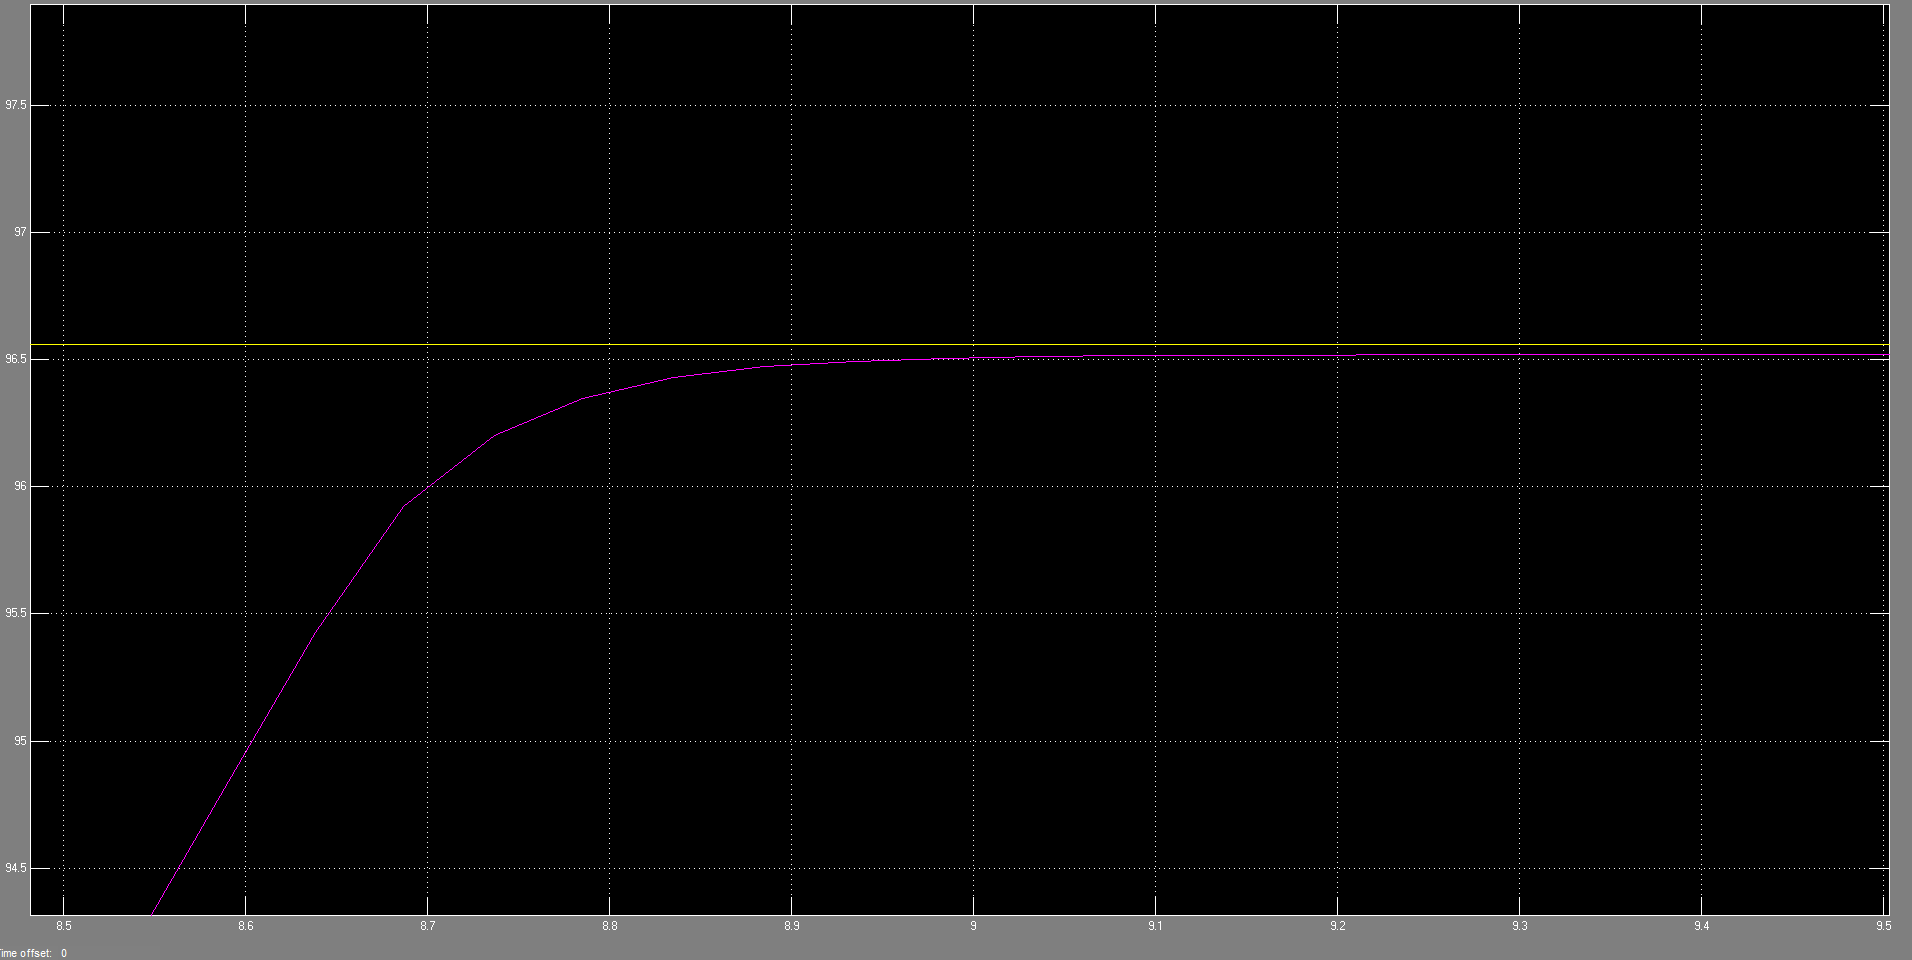
\includegraphics[scale = 0.27]{resources/Accelerationzoom.png}
\caption{The aerodynamic drag force.}
\label{fig:acceleration}
\end{figure}
\begin{figure}[H]
\centering
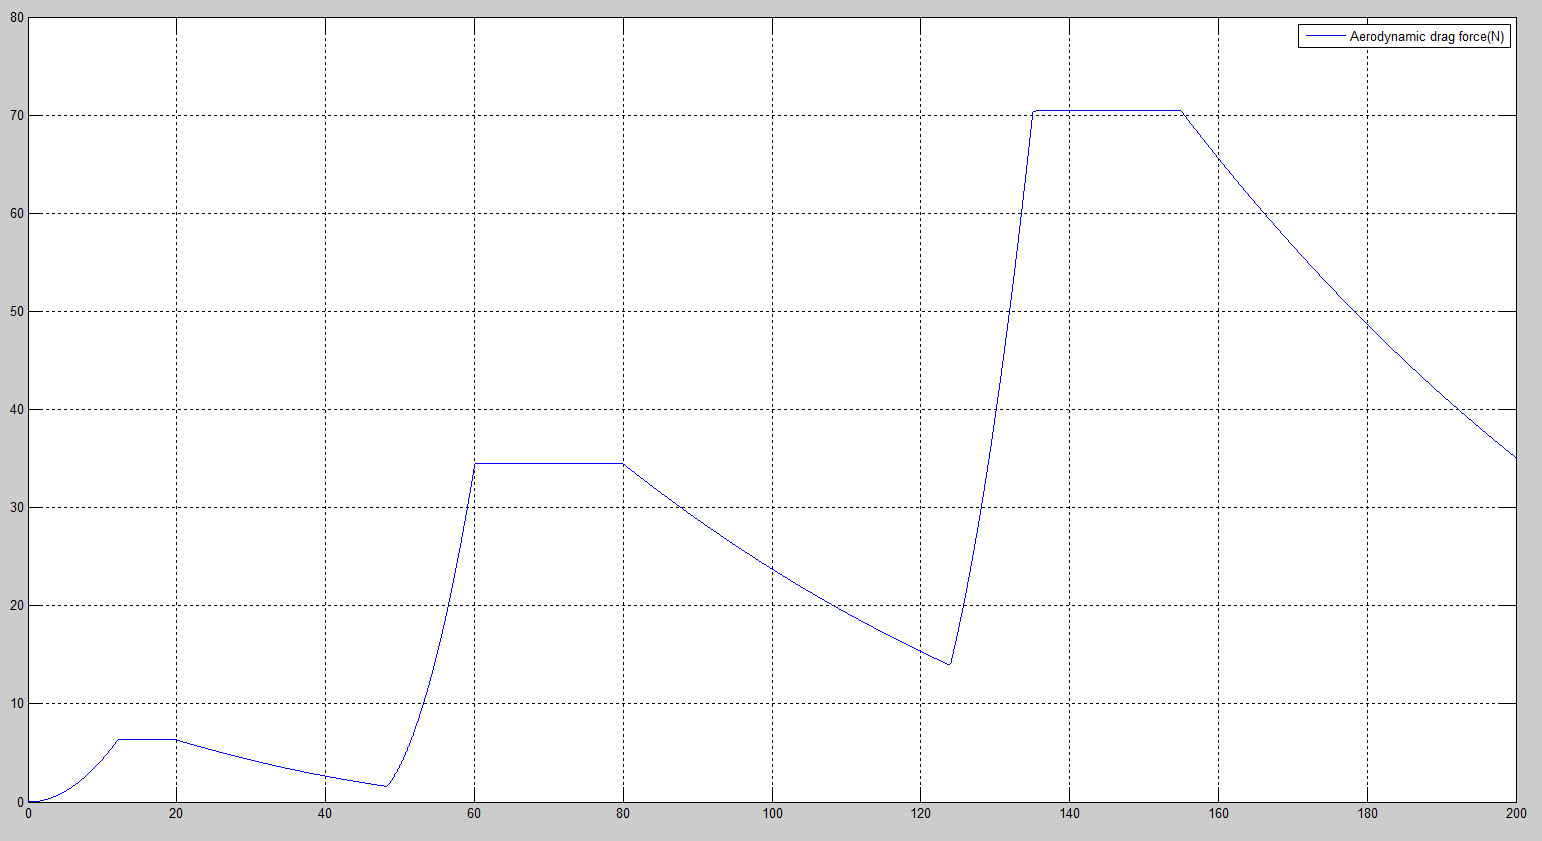
\includegraphics[scale = 0.27]{resources/Aerodynamic.png}
\caption{The aerodynamic drag force.}
\label{fig:Aerodynamic}
\end{figure}
As can be observed from \ref{fig:Aerodynamic}, a higher velocity will cause a higher aerodynamic drag force.
\begin{figure}[H]
\centering
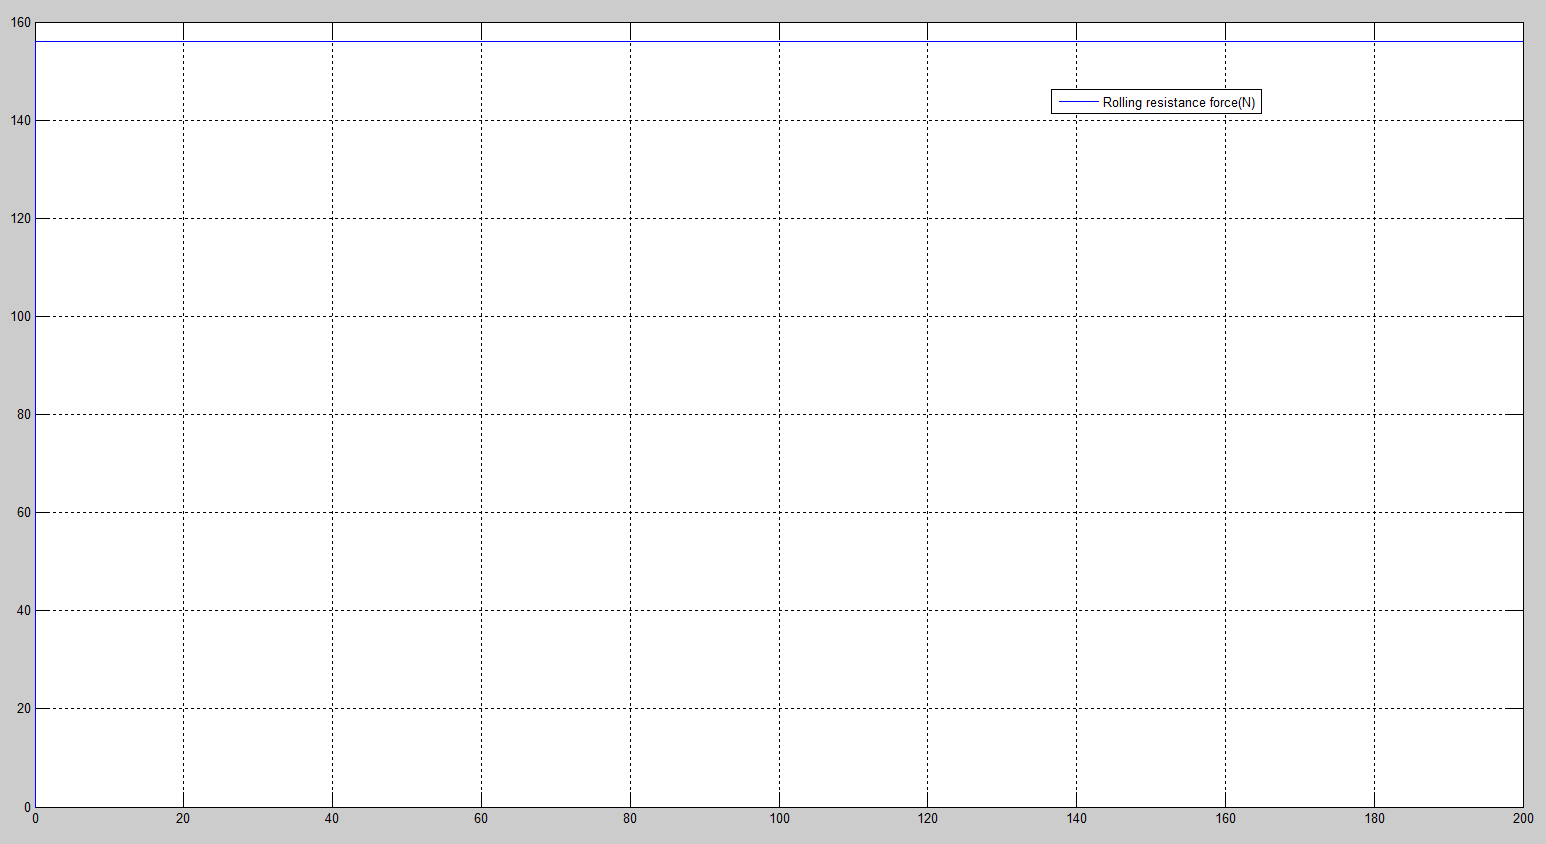
\includegraphics[scale = 0.27]{resources/Rolling.png}
\caption{The rolling resistance force.}
\label{fig:Rolling}
\end{figure}
The rolling resistance force is constant as the velocity has no influence.
\begin{figure}[H]
\centering
\includegraphics[trim = 0mm 35mm 60mm 0mm, clip, scale = 0.5]{resources/Wheeltorque.pdf}
\caption{Torque on the wheels.}
\label{fig:Wheeltorque}
\end{figure}
\begin{figure}[H]
\centering
\includegraphics[trim = 0mm 35mm 60mm 0mm, clip, scale = 0.5]{resources/Mot_torque.pdf}
\caption{Motor torque.}
\label{fig:Motortorque}
\end{figure}
During acceleration both the wheel torque, as well as the motor torque increase.
\begin{figure}[H]
\centering
\includegraphics[trim = 0mm 35mm 60mm 0mm, clip, scale = 0.5]{resources/Motorpower.pdf}
\caption{The motor output power.}
\label{fig:Motorpower}
\end{figure}
\begin{figure}[H]
\centering
\includegraphics[trim = 0mm 35mm 60mm 0mm, clip, scale = 0.5]{resources/Batterypower.pdf}
\caption{The battery output power.}
\label{fig:Batterypower}
\end{figure}
When torque is requested, the battery and motor output power increase.

\begin{figure}[H]
	\centering
	\newlength\figureheight 
	\newlength\figurewidth 
	\setlength\figureheight{4cm} 
	\setlength\figurewidth{0.8\linewidth}
	% This file was created by matlab2tikz v0.4.6 running on MATLAB 8.2.
% Copyright (c) 2008--2014, Nico Schlömer <nico.schloemer@gmail.com>
% All rights reserved.
% Minimal pgfplots version: 1.3
% 
% The latest updates can be retrieved from
%   http://www.mathworks.com/matlabcentral/fileexchange/22022-matlab2tikz
% where you can also make suggestions and rate matlab2tikz.
% 
\begin{tikzpicture}

\begin{axis}[%
width=\figurewidth,
height=\figureheight,
scale only axis,
xmin=0,
xmax=140,
ymin=0,
ymax=50000,
legend style={draw=black,fill=white,legend cell align=left}
]
\addplot [color=blue,solid]
  table[row sep=crcr]{
10	491.582968696133	\\
20	1029.83539576803	\\
30	1659.95206957162	\\
40	2427.89404693995	\\
50	3379.6083200908	\\
60	4561.0278724996	\\
70	6018.07173242414	\\
80	7796.64503463515	\\
90	9942.6390632613	\\
100	12501.9312463914	\\
110	15520.385082977	\\
120	19043.8500112867	\\
130	23118.1612622991	\\
140	27789.1397632865	\\
};
\addlegendentry{Power at 0\% incl.};

\addplot [color=black!50!green,solid]
  table[row sep=crcr]{
10	1933.11092704637	\\
20	3924.28750568366	\\
30	6007.03180608588	\\
40	8227.30588708286	\\
50	10631.0574563532	\\
60	13264.220100603	\\
70	16172.7132576758	\\
80	19402.4422012964	\\
90	22999.2980170646	\\
100	27009.1576023527	\\
110	31477.8836827581	\\
120	36451.3248675007	\\
130	41975.3157181301	\\
140	48095.6768150687	\\
};
\addlegendentry{Power at 3\% incl.};

\end{axis}
\end{tikzpicture}%
	\caption{Required power to main constant velocity.}
	\label{fig:req_power}
\end{figure}
At higher velocity's more average power is required. Driving on an incline will require more average power.

The longest driving range can be probably be expected if the car is driven at a low and constant velocity. No heavy luggage will also benefit the driving range.

\section{Task 2: Labotory electric car}

The lab car is about 6 kg and the frontal area = $25cm*20cm = 0.05 m^2$. Furthermore the wheels are modeled as four cylinders with a mass of 150g and a radius of 6.5 cm, therefore the moment of inertia is $1.264g*m^2$. The moment of inertia of the motor shaft is about $0.02g*m^2$, this is calculated using the model of two cylinders of about 50g with a radius of 1 cm. The rolling resistance coefficient is estimated to be 0.01 and the total efficiency is given to be 0.9. The total capacitance is 35F.

\begin{figure}[H]
	\centering
		\newlength\figureheight 
	\newlength\figurewidth 
    	\setlength\figureheight{4cm}
    	\setlength\figurewidth{0.8\linewidth}
    	% This file was created by matlab2tikz v0.4.6 running on MATLAB 8.2.
% Copyright (c) 2008--2014, Nico Schlömer <nico.schloemer@gmail.com>
% All rights reserved.
% Minimal pgfplots version: 1.3
% 
% The latest updates can be retrieved from
%   http://www.mathworks.com/matlabcentral/fileexchange/22022-matlab2tikz
% where you can also make suggestions and rate matlab2tikz.
% 
\begin{tikzpicture}

\begin{axis}[%
width=\figurewidth,
height=\figureheight,
scale only axis,
xmin=0,
xmax=200,
xmajorgrids,
ymin=0,
ymax=0.8,
ymajorgrids,
name=plot1,
legend style={draw=black,fill=white,legend cell align=left}
]
\addplot [color=blue,solid]
  table[row sep=crcr]{
0	0	\\
0	0	\\
0.0102533453420371	0.5886	\\
0.468710439722908	0.5886	\\
0.468710439722908	0.5886	\\
0.928710439722908	0.5886	\\
0.928710439722908	0.5886	\\
1.38871043972291	0.5886	\\
1.38871043972291	0.5886	\\
1.84871043972291	0.5886	\\
1.84871043972291	0.5886	\\
2.3087104397229	0.5886	\\
2.3087104397229	0.5886	\\
2.76871043972289	0.5886	\\
2.76871043972289	0.5886	\\
3.22871043972288	0.5886	\\
3.22871043972288	0.5886	\\
3.68871043972287	0.5886	\\
3.68871043972287	0.5886	\\
4.14871043972286	0.5886	\\
4.14871043972286	0.5886	\\
4.60871043972285	0.5886	\\
4.60871043972285	0.5886	\\
5.07871043972284	0.5886	\\
5.07871043972284	0.5886	\\
5.53871043972283	0.5886	\\
5.53871043972283	0.5886	\\
5.99871043972282	0.5886	\\
5.99871043972282	0.5886	\\
6.45871043972281	0.5886	\\
6.45871043972281	0.5886	\\
6.9187104397228	0.5886	\\
6.9187104397228	0.5886	\\
7.37871043972279	0.5886	\\
7.37871043972279	0.5886	\\
7.83871043972279	0.5886	\\
7.83871043972279	0.5886	\\
8.29871043972278	0.5886	\\
8.29871043972278	0.5886	\\
8.75871043972277	0.5886	\\
8.75871043972277	0.5886	\\
9.21871043972276	0.5886	\\
9.21871043972276	0.5886	\\
9.67871043972275	0.5886	\\
9.67871043972275	0.5886	\\
10.1387104397227	0.5886	\\
10.1387104397227	0.5886	\\
10.6087104397227	0.5886	\\
10.6087104397227	0.5886	\\
11.0687104397227	0.5886	\\
11.0687104397227	0.5886	\\
11.5287104397227	0.5886	\\
11.5287104397227	0.5886	\\
11.9887104397227	0.5886	\\
11.9887104397227	0.5886	\\
12.4487104397227	0.5886	\\
12.4487104397227	0.5886	\\
12.9087104397227	0.5886	\\
12.9087104397227	0.5886	\\
13.3687104397227	0.5886	\\
13.3687104397227	0.5886	\\
13.8287104397227	0.5886	\\
13.8287104397227	0.5886	\\
14.2887104397226	0.5886	\\
14.2887104397226	0.5886	\\
14.7487104397226	0.5886	\\
14.7487104397226	0.5886	\\
15.2087104397226	0.5886	\\
15.2087104397226	0.5886	\\
15.6687104397226	0.5886	\\
15.6687104397226	0.5886	\\
16.1387104397226	0.5886	\\
16.1387104397226	0.5886	\\
16.5987104397227	0.5886	\\
16.5987104397227	0.5886	\\
17.0587104397228	0.5886	\\
17.0587104397228	0.5886	\\
17.5187104397228	0.5886	\\
17.5187104397228	0.5886	\\
17.9787104397229	0.5886	\\
17.9787104397229	0.5886	\\
18.438710439723	0.5886	\\
18.438710439723	0.5886	\\
18.8987104397231	0.5886	\\
18.8987104397231	0.5886	\\
19.3587104397231	0.5886	\\
19.3587104397231	0.5886	\\
19.8187104397232	0.5886	\\
19.8187104397232	0.5886	\\
20.2819601478846	0.5886	\\
20.2819601478846	0.5886	\\
20.7419601478847	0.5886	\\
20.7419601478847	0.5886	\\
21.2019601478848	0.5886	\\
21.2019601478848	0.5886	\\
21.6619601478848	0.5886	\\
21.6619601478848	0.5886	\\
22.1219601478849	0.5886	\\
22.1219601478849	0.5886	\\
22.581960147885	0.5886	\\
22.581960147885	0.5886	\\
23.0419601478851	0.5886	\\
23.0419601478851	0.5886	\\
23.5119601478851	0.5886	\\
23.5119601478851	0.5886	\\
23.9719601478852	0.5886	\\
23.9719601478852	0.5886	\\
24.4319601478853	0.5886	\\
24.4319601478853	0.5886	\\
24.8919601478853	0.5886	\\
24.8919601478853	0.5886	\\
25.3519601478854	0.5886	\\
25.3519601478854	0.5886	\\
25.8119601478855	0.5886	\\
25.8119601478855	0.5886	\\
26.2719601478856	0.5886	\\
26.2719601478856	0.5886	\\
26.7319601478856	0.5886	\\
26.7319601478856	0.5886	\\
27.1919601478857	0.5886	\\
27.1919601478857	0.5886	\\
27.6519601478858	0.5886	\\
27.6519601478858	0.5886	\\
28.1119601478858	0.5886	\\
28.1119601478858	0.5886	\\
28.5719601478859	0.5886	\\
28.5719601478859	0.5886	\\
29.041960147886	0.5886	\\
29.041960147886	0.5886	\\
29.5019601478861	0.5886	\\
29.5019601478861	0.5886	\\
29.9619601478861	0.5886	\\
29.9619601478861	0.5886	\\
30.4219601478862	0.5886	\\
30.4219601478862	0.5886	\\
30.8819601478863	0.5886	\\
30.8819601478863	0.5886	\\
31.3419601478864	0.5886	\\
31.3419601478864	0.5886	\\
31.8019601478864	0.5886	\\
31.8019601478864	0.5886	\\
32.2619601478864	0.5886	\\
32.2619601478864	0.5886	\\
32.7219601478863	0.5886	\\
32.7219601478863	0.5886	\\
33.1819601478862	0.5886	\\
33.1819601478862	0.5886	\\
33.6419601478861	0.5886	\\
33.6419601478861	0.5886	\\
34.101960147886	0.5886	\\
34.101960147886	0.5886	\\
34.5719601478859	0.5886	\\
34.5719601478859	0.5886	\\
35.0319601478858	0.5886	\\
35.0319601478858	0.5886	\\
35.4919601478858	0.5886	\\
35.4919601478858	0.5886	\\
35.9519601478857	0.5886	\\
35.9519601478857	0.5886	\\
36.4119601478856	0.5886	\\
36.4119601478856	0.5886	\\
36.8719601478855	0.5886	\\
36.8719601478855	0.5886	\\
37.3319601478854	0.5886	\\
37.3319601478854	0.5886	\\
37.7919601478853	0.5886	\\
37.7919601478853	0.5886	\\
38.2519601478852	0.5886	\\
38.2519601478852	0.5886	\\
38.7119601478851	0.5886	\\
38.7119601478851	0.5886	\\
39.171960147885	0.5886	\\
39.171960147885	0.5886	\\
39.6319601478849	0.5886	\\
39.6319601478849	0.5886	\\
40.1000000000004	0.5886	\\
40.1000000000004	0.5886	\\
40.5600000000003	0.5886	\\
40.5600000000003	0.5886	\\
41.0200000000003	0.5886	\\
41.0200000000003	0.5886	\\
41.4800000000002	0.5886	\\
41.4800000000002	0.5886	\\
41.9400000000001	0.5886	\\
41.9400000000001	0.5886	\\
42.4	0.5886	\\
42.4	0.5886	\\
42.8599999999999	0.5886	\\
42.8599999999999	0.5886	\\
43.3199999999998	0.5886	\\
43.3199999999998	0.5886	\\
43.7799999999997	0.5886	\\
43.7799999999997	0.5886	\\
44.2399999999996	0.5886	\\
44.2399999999996	0.5886	\\
44.7099999999995	0.5886	\\
44.7099999999995	0.5886	\\
45.1699999999994	0.5886	\\
45.1699999999994	0.5886	\\
45.6299999999993	0.5886	\\
45.6299999999993	0.5886	\\
46.0899999999992	0.5886	\\
46.0899999999992	0.5886	\\
46.5499999999992	0.5886	\\
46.5499999999992	0.5886	\\
47.0099999999991	0.5886	\\
47.0099999999991	0.5886	\\
47.469999999999	0.5886	\\
47.469999999999	0.5886	\\
47.9299999999989	0.5886	\\
47.9299999999989	0.5886	\\
48.3899999999988	0.5886	\\
48.3899999999988	0.5886	\\
48.8499999999987	0.5886	\\
48.8499999999987	0.5886	\\
49.3099999999986	0.5886	\\
49.3099999999986	0.5886	\\
49.7709257472683	0.5886	\\
49.7709257472683	0.5886	\\
50.2309257472682	0.5886	\\
50.2309257472682	0.5886	\\
50.7009257472681	0.5886	\\
50.7009257472681	0.5886	\\
51.160925747268	0.5886	\\
51.160925747268	0.5886	\\
51.6209257472679	0.5886	\\
51.6209257472679	0.5886	\\
52.0809257472678	0.5886	\\
52.0809257472678	0.5886	\\
52.5409257472677	0.5886	\\
52.5409257472677	0.5886	\\
53.0009257472676	0.5886	\\
53.0009257472676	0.5886	\\
53.4609257472675	0.5886	\\
53.4609257472675	0.5886	\\
53.9209257472675	0.5886	\\
53.9209257472675	0.5886	\\
54.3809257472674	0.5886	\\
54.3809257472674	0.5886	\\
54.8409257472673	0.5886	\\
54.8409257472673	0.5886	\\
55.3009257472672	0.5886	\\
55.3009257472672	0.5886	\\
55.7609257472671	0.5886	\\
55.7609257472671	0.5886	\\
56.230925747267	0.5886	\\
56.230925747267	0.5886	\\
56.6909257472669	0.5886	\\
56.6909257472669	0.5886	\\
57.1509257472668	0.5886	\\
57.1509257472668	0.5886	\\
57.6109257472667	0.5886	\\
57.6109257472667	0.5886	\\
58.0709257472666	0.5886	\\
58.0709257472666	0.5886	\\
58.5309257472665	0.5886	\\
58.5309257472665	0.5886	\\
58.9909257472664	0.5886	\\
58.9909257472664	0.5886	\\
59.4509257472664	0.5886	\\
59.4509257472664	0.5886	\\
59.9109257472663	0.5886	\\
59.9109257472663	0.5886	\\
60.3700000000004	0.5886	\\
60.3700000000004	0.5886	\\
60.8300000000003	0.5886	\\
60.8300000000003	0.5886	\\
61.3000000000002	0.5886	\\
61.3000000000002	0.5886	\\
61.7600000000001	0.5886	\\
61.7600000000001	0.5886	\\
62.22	0.5886	\\
62.22	0.5886	\\
62.6799999999999	0.5886	\\
62.6799999999999	0.5886	\\
63.1399999999998	0.5886	\\
63.1399999999998	0.5886	\\
63.5999999999997	0.5886	\\
63.5999999999997	0.5886	\\
64.0599999999997	0.5886	\\
64.0599999999997	0.5886	\\
64.5199999999999	0.5886	\\
64.5199999999999	0.5886	\\
64.9800000000002	0.5886	\\
64.9800000000002	0.5886	\\
65.4400000000004	0.5886	\\
65.4400000000004	0.5886	\\
65.9000000000006	0.5886	\\
65.9000000000006	0.5886	\\
66.3600000000009	0.5886	\\
66.3600000000009	0.5886	\\
66.8300000000011	0.5886	\\
66.8300000000011	0.5886	\\
67.2900000000013	0.5886	\\
67.2900000000013	0.5886	\\
67.7500000000016	0.5886	\\
67.7500000000016	0.5886	\\
68.2100000000018	0.5886	\\
68.2100000000018	0.5886	\\
68.670000000002	0.5886	\\
68.670000000002	0.5886	\\
69.1300000000023	0.5886	\\
69.1300000000023	0.5886	\\
69.5900000000025	0.5886	\\
69.5900000000025	0.5886	\\
70.0500000000028	0.5886	\\
70.0500000000028	0.5886	\\
70.510000000003	0.5886	\\
70.510000000003	0.5886	\\
70.9700000000032	0.5886	\\
70.9700000000032	0.5886	\\
71.4300000000035	0.5886	\\
71.4300000000035	0.5886	\\
71.8900000000037	0.5886	\\
71.8900000000037	0.5886	\\
72.3600000000039	0.5886	\\
72.3600000000039	0.5886	\\
72.8200000000042	0.5886	\\
72.8200000000042	0.5886	\\
73.2800000000044	0.5886	\\
73.2800000000044	0.5886	\\
73.7400000000046	0.5886	\\
73.7400000000046	0.5886	\\
74.2000000000049	0.5886	\\
74.2000000000049	0.5886	\\
74.6600000000051	0.5886	\\
74.6600000000051	0.5886	\\
75.1200000000053	0.5886	\\
75.1200000000053	0.5886	\\
75.5800000000056	0.5886	\\
75.5800000000056	0.5886	\\
76.0400000000058	0.5886	\\
76.0400000000058	0.5886	\\
76.5000000000061	0.5886	\\
76.5000000000061	0.5886	\\
76.9600000000063	0.5886	\\
76.9600000000063	0.5886	\\
77.4200000000065	0.5886	\\
77.4200000000065	0.5886	\\
77.8900000000068	0.5886	\\
77.8900000000068	0.5886	\\
78.350000000007	0.5886	\\
78.350000000007	0.5886	\\
78.8100000000072	0.5886	\\
78.8100000000072	0.5886	\\
79.2700000000075	0.5886	\\
79.2700000000075	0.5886	\\
79.7300000000077	0.5886	\\
79.7300000000077	0.5886	\\
80.1874566251345	0.5886	\\
80.1874566251345	0.5886	\\
80.6474566251348	0.5886	\\
80.6474566251348	0.5886	\\
81.107456625135	0.5886	\\
81.107456625135	0.5886	\\
81.5674566251353	0.5886	\\
81.5674566251353	0.5886	\\
82.0374566251355	0.5886	\\
82.0374566251355	0.5886	\\
82.4974566251357	0.5886	\\
82.4974566251357	0.5886	\\
82.957456625136	0.5886	\\
82.957456625136	0.5886	\\
83.4174566251362	0.5886	\\
83.4174566251362	0.5886	\\
83.8774566251364	0.5886	\\
83.8774566251364	0.5886	\\
84.3374566251367	0.5886	\\
84.3374566251367	0.5886	\\
84.7974566251369	0.5886	\\
84.7974566251369	0.5886	\\
85.2574566251371	0.5886	\\
85.2574566251371	0.5886	\\
85.7174566251374	0.5886	\\
85.7174566251374	0.5886	\\
86.1774566251376	0.5886	\\
86.1774566251376	0.5886	\\
86.6374566251378	0.5886	\\
86.6374566251378	0.5886	\\
87.0974566251381	0.5886	\\
87.0974566251381	0.5886	\\
87.5674566251383	0.5886	\\
87.5674566251383	0.5886	\\
88.0274566251386	0.5886	\\
88.0274566251386	0.5886	\\
88.4874566251388	0.5886	\\
88.4874566251388	0.5886	\\
88.947456625139	0.5886	\\
88.947456625139	0.5886	\\
89.4074566251393	0.5886	\\
89.4074566251393	0.5886	\\
89.8674566251395	0.5886	\\
89.8674566251395	0.5886	\\
90.3274566251397	0.5886	\\
90.3274566251397	0.5886	\\
90.78745662514	0.5886	\\
90.78745662514	0.5886	\\
91.2474566251402	0.5886	\\
91.2474566251402	0.5886	\\
91.7074566251404	0.5886	\\
91.7074566251404	0.5886	\\
92.1674566251407	0.5886	\\
92.1674566251407	0.5886	\\
92.6274566251409	0.5886	\\
92.6274566251409	0.5886	\\
93.0974566251411	0.5886	\\
93.0974566251411	0.5886	\\
93.5574566251414	0.5886	\\
93.5574566251414	0.5886	\\
94.0174566251416	0.5886	\\
94.0174566251416	0.5886	\\
94.4774566251419	0.5886	\\
94.4774566251419	0.5886	\\
94.9374566251421	0.5886	\\
94.9374566251421	0.5886	\\
95.3974566251423	0.5886	\\
95.3974566251423	0.5886	\\
95.8574566251426	0.5886	\\
95.8574566251426	0.5886	\\
96.3174566251428	0.5886	\\
96.3174566251428	0.5886	\\
96.777456625143	0.5886	\\
96.777456625143	0.5886	\\
97.2374566251433	0.5886	\\
97.2374566251433	0.5886	\\
97.6974566251435	0.5886	\\
97.6974566251435	0.5886	\\
98.1574566251437	0.5886	\\
98.1574566251437	0.5886	\\
98.627456625144	0.5886	\\
98.627456625144	0.5886	\\
99.0874566251442	0.5886	\\
99.0874566251442	0.5886	\\
99.5474566251444	0.5886	\\
99.5474566251444	0.5886	\\
100.007456625145	0.5886	\\
100.007456625145	0.5886	\\
100.467456625145	0.5886	\\
100.467456625145	0.5886	\\
100.927456625145	0.5886	\\
100.927456625145	0.5886	\\
101.387456625145	0.5886	\\
101.387456625145	0.5886	\\
101.847456625146	0.5886	\\
101.847456625146	0.5886	\\
102.307456625146	0.5886	\\
102.307456625146	0.5886	\\
102.767456625146	0.5886	\\
102.767456625146	0.5886	\\
103.227456625146	0.5886	\\
103.227456625146	0.5886	\\
103.687456625147	0.5886	\\
103.687456625147	0.5886	\\
104.157456625147	0.5886	\\
104.157456625147	0.5886	\\
104.617456625147	0.5886	\\
104.617456625147	0.5886	\\
105.077456625147	0.5886	\\
105.077456625147	0.5886	\\
105.537456625148	0.5886	\\
105.537456625148	0.5886	\\
105.997456625148	0.5886	\\
105.997456625148	0.5886	\\
106.457456625148	0.5886	\\
106.457456625148	0.5886	\\
106.917456625148	0.5886	\\
106.917456625148	0.5886	\\
107.377456625148	0.5886	\\
107.377456625148	0.5886	\\
107.837456625149	0.5886	\\
107.837456625149	0.5886	\\
108.297456625149	0.5886	\\
108.297456625149	0.5886	\\
108.757456625149	0.5886	\\
108.757456625149	0.5886	\\
109.217456625149	0.5886	\\
109.217456625149	0.5886	\\
109.67745662515	0.5886	\\
109.67745662515	0.5886	\\
110.14745662515	0.5886	\\
110.14745662515	0.5886	\\
110.60745662515	0.5886	\\
110.60745662515	0.5886	\\
111.06745662515	0.5886	\\
111.06745662515	0.5886	\\
111.527456625151	0.5886	\\
111.527456625151	0.5886	\\
111.987456625151	0.5886	\\
111.987456625151	0.5886	\\
112.447456625151	0.5886	\\
112.447456625151	0.5886	\\
112.907456625151	0.5886	\\
112.907456625151	0.5886	\\
113.367456625152	0.5886	\\
113.367456625152	0.5886	\\
113.827456625152	0.5886	\\
113.827456625152	0.5886	\\
114.287456625152	0.5886	\\
114.287456625152	0.5886	\\
114.747456625152	0.5886	\\
114.747456625152	0.5886	\\
115.207456625152	0.5886	\\
115.207456625152	0.5886	\\
115.677456625153	0.5886	\\
115.677456625153	0.5886	\\
116.137456625153	0.5886	\\
116.137456625153	0.5886	\\
116.597456625153	0.5886	\\
116.597456625153	0.5886	\\
117.057456625153	0.5886	\\
117.057456625153	0.5886	\\
117.517456625154	0.5886	\\
117.517456625154	0.5886	\\
117.977456625154	0.5886	\\
117.977456625154	0.5886	\\
118.437456625154	0.5886	\\
118.437456625154	0.5886	\\
118.897456625154	0.5886	\\
118.897456625154	0.5886	\\
119.357456625155	0.5886	\\
119.357456625155	0.5886	\\
119.817456625155	0.5886	\\
119.817456625155	0.5886	\\
120.277456625155	0.5886	\\
120.277456625155	0.5886	\\
120.737456625155	0.5886	\\
120.737456625155	0.5886	\\
121.207456625156	0.5886	\\
121.207456625156	0.5886	\\
121.667456625156	0.5886	\\
121.667456625156	0.5886	\\
122.127456625156	0.5886	\\
122.127456625156	0.5886	\\
122.587456625156	0.5886	\\
122.587456625156	0.5886	\\
123.047456625156	0.5886	\\
123.047456625156	0.5886	\\
123.507456625157	0.5886	\\
123.507456625157	0.5886	\\
123.967456625157	0.5886	\\
123.967456625157	0.5886	\\
124.428701160911	0.5886	\\
124.428701160911	0.5886	\\
124.888701160911	0.5886	\\
124.888701160911	0.5886	\\
125.348701160911	0.5886	\\
125.348701160911	0.5886	\\
125.808701160911	0.5886	\\
125.808701160911	0.5886	\\
126.268701160912	0.5886	\\
126.268701160912	0.5886	\\
126.728701160912	0.5886	\\
126.728701160912	0.5886	\\
127.198701160912	0.5886	\\
127.198701160912	0.5886	\\
127.658701160912	0.5886	\\
127.658701160912	0.5886	\\
128.118701160912	0.5886	\\
128.118701160912	0.5886	\\
128.578701160912	0.5886	\\
128.578701160912	0.5886	\\
129.038701160912	0.5886	\\
129.038701160912	0.5886	\\
129.498701160911	0.5886	\\
129.498701160911	0.5886	\\
129.958701160911	0.5886	\\
129.958701160911	0.5886	\\
130.41870116091	0.5886	\\
130.41870116091	0.5886	\\
130.87870116091	0.5886	\\
130.87870116091	0.5886	\\
131.338701160909	0.5886	\\
131.338701160909	0.5886	\\
131.798701160909	0.5886	\\
131.798701160909	0.5886	\\
132.258701160909	0.5886	\\
132.258701160909	0.5886	\\
132.728701160908	0.5886	\\
132.728701160908	0.5886	\\
133.188701160908	0.5886	\\
133.188701160908	0.5886	\\
133.648701160907	0.5886	\\
133.648701160907	0.5886	\\
134.108701160907	0.5886	\\
134.108701160907	0.5886	\\
134.568701160907	0.5886	\\
134.568701160907	0.5886	\\
135.028701160906	0.5886	\\
135.028701160906	0.5886	\\
135.488701160906	0.5886	\\
135.488701160906	0.5886	\\
135.948701160905	0.5886	\\
135.948701160905	0.5886	\\
136.408701160905	0.5886	\\
136.408701160905	0.5886	\\
136.868701160904	0.5886	\\
136.868701160904	0.5886	\\
137.328701160904	0.5886	\\
137.328701160904	0.5886	\\
137.788701160904	0.5886	\\
137.788701160904	0.5886	\\
138.258701160903	0.5886	\\
138.258701160903	0.5886	\\
138.718701160903	0.5886	\\
138.718701160903	0.5886	\\
139.178701160902	0.5886	\\
139.178701160902	0.5886	\\
139.638701160902	0.5886	\\
139.638701160902	0.5886	\\
140.098701160902	0.5886	\\
140.098701160902	0.5886	\\
140.558701160901	0.5886	\\
140.558701160901	0.5886	\\
141.018701160901	0.5886	\\
141.018701160901	0.5886	\\
141.4787011609	0.5886	\\
141.4787011609	0.5886	\\
141.9387011609	0.5886	\\
141.9387011609	0.5886	\\
142.398701160899	0.5886	\\
142.398701160899	0.5886	\\
142.858701160899	0.5886	\\
142.858701160899	0.5886	\\
143.318701160899	0.5886	\\
143.318701160899	0.5886	\\
143.788701160898	0.5886	\\
143.788701160898	0.5886	\\
144.248701160898	0.5886	\\
144.248701160898	0.5886	\\
144.708701160897	0.5886	\\
144.708701160897	0.5886	\\
145.168701160897	0.5886	\\
145.168701160897	0.5886	\\
145.628701160897	0.5886	\\
145.628701160897	0.5886	\\
146.088701160896	0.5886	\\
146.088701160896	0.5886	\\
146.548701160896	0.5886	\\
146.548701160896	0.5886	\\
147.008701160895	0.5886	\\
147.008701160895	0.5886	\\
147.468701160895	0.5886	\\
147.468701160895	0.5886	\\
147.928701160894	0.5886	\\
147.928701160894	0.5886	\\
148.388701160894	0.5886	\\
148.388701160894	0.5886	\\
148.848701160894	0.5886	\\
148.848701160894	0.5886	\\
149.318701160893	0.5886	\\
149.318701160893	0.5886	\\
149.778701160893	0.5886	\\
149.778701160893	0.5886	\\
150.238701160892	0.5886	\\
150.238701160892	0.5886	\\
150.698701160892	0.5886	\\
150.698701160892	0.5886	\\
151.158701160891	0.5886	\\
151.158701160891	0.5886	\\
151.618701160891	0.5886	\\
151.618701160891	0.5886	\\
152.078701160891	0.5886	\\
152.078701160891	0.5886	\\
152.53870116089	0.5886	\\
152.53870116089	0.5886	\\
152.99870116089	0.5886	\\
152.99870116089	0.5886	\\
153.458701160889	0.5886	\\
153.458701160889	0.5886	\\
153.918701160889	0.5886	\\
153.918701160889	0.5886	\\
154.378701160889	0.5886	\\
154.378701160889	0.5886	\\
154.848701160888	0.5886	\\
154.848701160888	0.5886	\\
155.30337472355	0.5886	\\
155.30337472355	0.5886	\\
155.763374723549	0.5886	\\
155.763374723549	0.5886	\\
156.223374723549	0.5886	\\
156.223374723549	0.5886	\\
156.683374723548	0.5886	\\
156.683374723548	0.5886	\\
157.143374723548	0.5886	\\
157.143374723548	0.5886	\\
157.613374723548	0.5886	\\
157.613374723548	0.5886	\\
158.073374723547	0.5886	\\
158.073374723547	0.5886	\\
158.533374723547	0.5886	\\
158.533374723547	0.5886	\\
158.993374723546	0.5886	\\
158.993374723546	0.5886	\\
159.453374723546	0.5886	\\
159.453374723546	0.5886	\\
159.913374723546	0.5886	\\
159.913374723546	0.5886	\\
160.373374723545	0.5886	\\
160.373374723545	0.5886	\\
160.833374723545	0.5886	\\
160.833374723545	0.5886	\\
161.293374723544	0.5886	\\
161.293374723544	0.5886	\\
161.753374723544	0.5886	\\
161.753374723544	0.5886	\\
162.213374723543	0.5886	\\
162.213374723543	0.5886	\\
162.673374723543	0.5886	\\
162.673374723543	0.5886	\\
163.143374723543	0.5886	\\
163.143374723543	0.5886	\\
163.603374723542	0.5886	\\
163.603374723542	0.5886	\\
164.063374723542	0.5886	\\
164.063374723542	0.5886	\\
164.523374723541	0.5886	\\
164.523374723541	0.5886	\\
164.983374723541	0.5886	\\
164.983374723541	0.5886	\\
165.44337472354	0.5886	\\
165.44337472354	0.5886	\\
165.90337472354	0.5886	\\
165.90337472354	0.5886	\\
166.36337472354	0.5886	\\
166.36337472354	0.5886	\\
166.823374723539	0.5886	\\
166.823374723539	0.5886	\\
167.283374723539	0.5886	\\
167.283374723539	0.5886	\\
167.743374723538	0.5886	\\
167.743374723538	0.5886	\\
168.203374723538	0.5886	\\
168.203374723538	0.5886	\\
168.673374723538	0.5886	\\
168.673374723538	0.5886	\\
169.133374723537	0.5886	\\
169.133374723537	0.5886	\\
169.593374723537	0.5886	\\
169.593374723537	0.5886	\\
170.053374723536	0.5886	\\
170.053374723536	0.5886	\\
170.513374723536	0.5886	\\
170.513374723536	0.5886	\\
170.973374723535	0.5886	\\
170.973374723535	0.5886	\\
171.433374723535	0.5886	\\
171.433374723535	0.5886	\\
171.893374723535	0.5886	\\
171.893374723535	0.5886	\\
172.353374723534	0.5886	\\
172.353374723534	0.5886	\\
172.813374723534	0.5886	\\
172.813374723534	0.5886	\\
173.273374723533	0.5886	\\
173.273374723533	0.5886	\\
173.733374723533	0.5886	\\
173.733374723533	0.5886	\\
174.203374723533	0.5886	\\
174.203374723533	0.5886	\\
174.663374723532	0.5886	\\
174.663374723532	0.5886	\\
175.123374723532	0.5886	\\
175.123374723532	0.5886	\\
175.583374723531	0.5886	\\
175.583374723531	0.5886	\\
176.043374723531	0.5886	\\
176.043374723531	0.5886	\\
176.50337472353	0.5886	\\
176.50337472353	0.5886	\\
176.96337472353	0.5886	\\
176.96337472353	0.5886	\\
177.42337472353	0.5886	\\
177.42337472353	0.5886	\\
177.883374723529	0.5886	\\
177.883374723529	0.5886	\\
178.343374723529	0.5886	\\
178.343374723529	0.5886	\\
178.803374723528	0.5886	\\
178.803374723528	0.5886	\\
179.263374723528	0.5886	\\
179.263374723528	0.5886	\\
179.733374723527	0.5886	\\
179.733374723527	0.5886	\\
180.193374723527	0.5886	\\
180.193374723527	0.5886	\\
180.653374723527	0.5886	\\
180.653374723527	0.5886	\\
181.113374723526	0.5886	\\
181.113374723526	0.5886	\\
181.573374723526	0.5886	\\
181.573374723526	0.5886	\\
182.033374723525	0.5886	\\
182.033374723525	0.5886	\\
182.493374723525	0.5886	\\
182.493374723525	0.5886	\\
182.953374723525	0.5886	\\
182.953374723525	0.5886	\\
183.413374723524	0.5886	\\
183.413374723524	0.5886	\\
183.873374723524	0.5886	\\
183.873374723524	0.5886	\\
184.333374723523	0.5886	\\
184.333374723523	0.5886	\\
184.793374723523	0.5886	\\
184.793374723523	0.5886	\\
185.263374723522	0.5886	\\
185.263374723522	0.5886	\\
185.723374723522	0.5886	\\
185.723374723522	0.5886	\\
186.183374723522	0.5886	\\
186.183374723522	0.5886	\\
186.643374723521	0.5886	\\
186.643374723521	0.5886	\\
187.103374723521	0.5886	\\
187.103374723521	0.5886	\\
187.56337472352	0.5886	\\
187.56337472352	0.5886	\\
188.02337472352	0.5886	\\
188.02337472352	0.5886	\\
188.48337472352	0.5886	\\
188.48337472352	0.5886	\\
188.943374723519	0.5886	\\
188.943374723519	0.5886	\\
189.403374723519	0.5886	\\
189.403374723519	0.5886	\\
189.863374723518	0.5886	\\
189.863374723518	0.5886	\\
190.323374723518	0.5886	\\
190.323374723518	0.5886	\\
190.793374723517	0.5886	\\
190.793374723517	0.5886	\\
191.253374723517	0.5886	\\
191.253374723517	0.5886	\\
191.713374723517	0.5886	\\
191.713374723517	0.5886	\\
192.173374723516	0.5886	\\
192.173374723516	0.5886	\\
192.633374723516	0.5886	\\
192.633374723516	0.5886	\\
193.093374723515	0.5886	\\
193.093374723515	0.5886	\\
193.553374723515	0.5886	\\
193.553374723515	0.5886	\\
194.013374723514	0.5886	\\
194.013374723514	0.5886	\\
194.473374723514	0.5886	\\
194.473374723514	0.5886	\\
194.933374723514	0.5886	\\
194.933374723514	0.5886	\\
195.393374723513	0.5886	\\
195.393374723513	0.5886	\\
195.853374723513	0.5886	\\
195.853374723513	0.5886	\\
196.313374723512	0.5886	\\
196.313374723512	0.5886	\\
196.783374723512	0.5886	\\
196.783374723512	0.5886	\\
197.243374723512	0.5886	\\
197.243374723512	0.5886	\\
197.703374723511	0.5886	\\
197.703374723511	0.5886	\\
198.163374723511	0.5886	\\
198.163374723511	0.5886	\\
198.62337472351	0.5886	\\
198.62337472351	0.5886	\\
199.08337472351	0.5886	\\
199.08337472351	0.5886	\\
200	0.5886	\\
};
\addlegendentry{Rolling resistance F (N)};

\end{axis}

\begin{axis}[%
width=\figurewidth,
height=\figureheight,
scale only axis,
xmin=0,
xmax=200,
xmajorgrids,
ymin=0,
ymax=2.5,
ymajorgrids,
at=(plot1.below south west),
anchor=above north west,
legend style={draw=black,fill=white,legend cell align=left}
]
\addplot [color=blue,solid]
  table[row sep=crcr]{
0	0	\\
0	0	\\
0.468710439722908	0.000310124901108281	\\
0.468710439722908	0.000310124901108281	\\
0.928710439722908	0.00123250335337303	\\
0.928710439722908	0.00123250335337303	\\
1.38871043972291	0.00276714623365154	\\
1.38871043972291	0.00276714623365154	\\
1.84871043972291	0.00491405149560195	\\
1.84871043972291	0.00491405149560195	\\
2.3087104397229	0.0076732170928937	\\
2.3087104397229	0.0076732170928937	\\
2.76871043972289	0.0110446409792077	\\
2.76871043972289	0.0110446409792077	\\
3.22871043972288	0.0150283211082364	\\
3.22871043972288	0.0150283211082364	\\
3.68871043972287	0.0196242554336833	\\
3.68871043972287	0.0196242554336833	\\
4.14871043972286	0.0248324419092637	\\
4.14871043972286	0.0248324419092637	\\
4.60871043972285	0.030652878488704	\\
4.60871043972285	0.030652878488704	\\
5.07871043972284	0.03723220362208	\\
5.07871043972284	0.03723220362208	\\
5.53871043972283	0.0442904439436388	\\
5.53871043972283	0.0442904439436388	\\
5.99871043972282	0.0519609281858222	\\
5.99871043972282	0.0519609281858222	\\
6.45871043972281	0.0602436543024024	\\
6.45871043972281	0.0602436543024024	\\
6.9187104397228	0.0691386202471632	\\
6.9187104397228	0.0691386202471632	\\
7.37871043972279	0.0786458239738999	\\
7.37871043972279	0.0786458239738999	\\
7.83871043972279	0.0887652634364187	\\
7.83871043972279	0.0887652634364187	\\
8.29871043972278	0.0994969365885379	\\
8.29871043972278	0.0994969365885379	\\
8.75871043972277	0.110840841384087	\\
8.75871043972277	0.110840841384087	\\
9.21871043972276	0.122796975776906	\\
9.21871043972276	0.122796975776906	\\
9.67871043972275	0.135365337720847	\\
9.67871043972275	0.135365337720847	\\
10.1387104397227	0.148545925169775	\\
10.1387104397227	0.148545925169775	\\
10.6087104397227	0.162645379045728	\\
10.6087104397227	0.162645379045728	\\
11.0687104397227	0.177063720504686	\\
11.0687104397227	0.177063720504686	\\
11.5287104397227	0.19209428128581	\\
11.5287104397227	0.19209428128581	\\
11.9887104397227	0.207737059343007	\\
11.9887104397227	0.207737059343007	\\
12.1787104397227	0.208310173162708	\\
12.4487104397227	0.208310173162708	\\
12.4487104397227	0.208310173162708	\\
12.9087104397227	0.208310173162708	\\
12.9087104397227	0.208310173162708	\\
13.3687104397227	0.208310173162708	\\
13.3687104397227	0.208310173162708	\\
13.8287104397227	0.208310173162708	\\
13.8287104397227	0.208310173162708	\\
14.2887104397226	0.208310173162708	\\
14.2887104397226	0.208310173162708	\\
14.7487104397226	0.208310173162708	\\
14.7487104397226	0.208310173162708	\\
15.2087104397226	0.208310173162708	\\
15.2087104397226	0.208310173162708	\\
15.6687104397226	0.208310173162708	\\
15.6687104397226	0.208310173162708	\\
16.1387104397226	0.208310173162708	\\
16.1387104397226	0.208310173162708	\\
16.5987104397227	0.208310173162708	\\
16.5987104397227	0.208310173162708	\\
17.0587104397228	0.208310173162708	\\
17.0587104397228	0.208310173162708	\\
17.5187104397228	0.208310173162708	\\
17.5187104397228	0.208310173162708	\\
17.9787104397229	0.208310173162708	\\
17.9787104397229	0.208310173162708	\\
18.438710439723	0.208310173162708	\\
18.438710439723	0.208310173162708	\\
18.8987104397231	0.208310173162708	\\
18.8987104397231	0.208310173162708	\\
19.3587104397231	0.208310173162708	\\
19.3587104397231	0.208310173162708	\\
19.8187104397232	0.208310173162708	\\
20.2819601478846	0.207058799285837	\\
20.2819601478846	0.207058799285837	\\
20.7419601478847	0.20503829778534	\\
20.7419601478847	0.20503829778534	\\
21.2019601478848	0.20303278352954	\\
21.2019601478848	0.20303278352954	\\
21.6619601478848	0.201042143923759	\\
21.6619601478848	0.201042143923759	\\
22.1219601478849	0.199066267582823	\\
22.1219601478849	0.199066267582823	\\
22.581960147885	0.1971050443165	\\
22.581960147885	0.1971050443165	\\
23.0419601478851	0.195158365115145	\\
23.0419601478851	0.195158365115145	\\
23.5119601478851	0.193184276379441	\\
23.5119601478851	0.193184276379441	\\
23.9719601478852	0.19126667326612	\\
23.9719601478852	0.19126667326612	\\
24.4319601478853	0.189363291849871	\\
24.4319601478853	0.189363291849871	\\
24.8919601478853	0.187474027728297	\\
24.8919601478853	0.187474027728297	\\
25.3519601478854	0.185598777610586	\\
25.3519601478854	0.185598777610586	\\
25.8119601478855	0.183737439304363	\\
25.8119601478855	0.183737439304363	\\
26.2719601478856	0.181889911702726	\\
26.2719601478856	0.181889911702726	\\
26.7319601478856	0.180056094771468	\\
26.7319601478856	0.180056094771468	\\
27.1919601478857	0.17823588953648	\\
27.1919601478857	0.17823588953648	\\
27.6519601478858	0.176429198071336	\\
27.6519601478858	0.176429198071336	\\
28.1119601478858	0.17463592348505	\\
28.1119601478858	0.17463592348505	\\
28.5719601478859	0.172855969910014	\\
28.5719601478859	0.172855969910014	\\
29.041960147886	0.17105098155583	\\
29.041960147886	0.17105098155583	\\
29.5019601478861	0.169297670884481	\\
29.5019601478861	0.169297670884481	\\
29.9619601478861	0.167557397635712	\\
29.9619601478861	0.167557397635712	\\
30.4219601478862	0.165830069939245	\\
30.4219601478862	0.165830069939245	\\
30.8819601478863	0.164115596890111	\\
30.8819601478863	0.164115596890111	\\
31.3419601478864	0.162413888537582	\\
31.3419601478864	0.162413888537582	\\
31.8019601478864	0.16072485587424	\\
31.8019601478864	0.16072485587424	\\
32.2619601478864	0.159048410825218	\\
32.2619601478864	0.159048410825218	\\
32.7219601478863	0.157384466237574	\\
32.7219601478863	0.157384466237574	\\
33.1819601478862	0.155732935869827	\\
33.1819601478862	0.155732935869827	\\
33.6419601478861	0.154093734381634	\\
33.6419601478861	0.154093734381634	\\
34.101960147886	0.152466777323603	\\
34.101960147886	0.152466777323603	\\
34.5719601478859	0.150817011298433	\\
34.5719601478859	0.150817011298433	\\
35.0319601478858	0.149214554923159	\\
35.0319601478858	0.149214554923159	\\
35.4919601478858	0.147624093106373	\\
35.4919601478858	0.147624093106373	\\
35.9519601478857	0.146045544881918	\\
35.9519601478857	0.146045544881918	\\
36.4119601478856	0.144478830125566	\\
36.4119601478856	0.144478830125566	\\
36.8719601478855	0.142923869545664	\\
36.8719601478855	0.142923869545664	\\
37.3319601478854	0.141380584673895	\\
37.3319601478854	0.141380584673895	\\
37.7919601478853	0.139848897856182	\\
37.7919601478853	0.139848897856182	\\
38.2519601478852	0.138328732243705	\\
38.2519601478852	0.138328732243705	\\
38.7119601478851	0.136820011784045	\\
38.7119601478851	0.136820011784045	\\
39.171960147885	0.13532266121245	\\
39.171960147885	0.13532266121245	\\
39.6319601478849	0.133836606043221	\\
39.6319601478849	0.133836606043221	\\
40.1000000000004	0.13233609485365	\\
40.1000000000004	0.13233609485365	\\
40.5600000000003	0.130872604318638	\\
40.5600000000003	0.130872604318638	\\
41.0200000000003	0.129420189063577	\\
41.0200000000003	0.129420189063577	\\
41.4800000000002	0.127978777648116	\\
41.4800000000002	0.127978777648116	\\
41.9400000000001	0.126548299369474	\\
41.9400000000001	0.126548299369474	\\
42.4	0.125128684254504	\\
42.4	0.125128684254504	\\
42.8599999999999	0.12371986305187	\\
42.8599999999999	0.12371986305187	\\
43.3199999999998	0.122321767224327	\\
43.3199999999998	0.122321767224327	\\
43.7799999999997	0.120934328941106	\\
43.7799999999997	0.120934328941106	\\
44.2399999999996	0.119557481070402	\\
44.2399999999996	0.119557481070402	\\
44.7099999999995	0.118161570862893	\\
44.7099999999995	0.118161570862893	\\
45.1699999999994	0.116805931808036	\\
45.1699999999994	0.116805931808036	\\
45.6299999999993	0.115460684483158	\\
45.6299999999993	0.115460684483158	\\
46.0899999999992	0.114125764493676	\\
46.0899999999992	0.114125764493676	\\
46.5499999999992	0.112801108107751	\\
46.5499999999992	0.112801108107751	\\
47.0099999999991	0.111486652249363	\\
47.0099999999991	0.111486652249363	\\
47.469999999999	0.110182334491478	\\
47.469999999999	0.110182334491478	\\
47.9299999999989	0.108888093049309	\\
47.9299999999989	0.108888093049309	\\
48.3899999999988	0.107603866773671	\\
48.3899999999988	0.107603866773671	\\
48.8499999999987	0.106329595144412	\\
48.8499999999987	0.106329595144412	\\
49.3099999999986	0.105065218263947	\\
49.5509257472683	0.104406927232523	\\
49.7709257472683	0.114478828116305	\\
49.7709257472683	0.114478828116305	\\
50.2309257472682	0.137646162125312	\\
50.2309257472682	0.137646162125312	\\
50.7009257472681	0.163520465333125	\\
50.7009257472681	0.163520465333125	\\
51.160925747268	0.191000690009985	\\
51.160925747268	0.191000690009985	\\
51.6209257472679	0.220614152329181	\\
51.6209257472679	0.220614152329181	\\
52.0809257472678	0.252360838982432	\\
52.0809257472678	0.252360838982432	\\
52.5409257472677	0.286240736661598	\\
52.5409257472677	0.286240736661598	\\
53.0009257472676	0.322253832058677	\\
53.0009257472676	0.322253832058677	\\
53.4609257472675	0.360400111865802	\\
53.4609257472675	0.360400111865802	\\
53.9209257472675	0.40067956277525	\\
53.9209257472675	0.40067956277525	\\
54.3809257472674	0.44309217147943	\\
54.3809257472674	0.44309217147943	\\
54.8409257472673	0.487637924670894	\\
54.8409257472673	0.487637924670894	\\
55.3009257472672	0.534316809042331	\\
55.3009257472672	0.534316809042331	\\
55.7609257472671	0.583128811286569	\\
55.7609257472671	0.583128811286569	\\
56.230925747267	0.635205110279849	\\
56.230925747267	0.635205110279849	\\
56.6909257472669	0.688329679750045	\\
56.6909257472669	0.688329679750045	\\
57.1509257472668	0.743587326883077	\\
57.1509257472668	0.743587326883077	\\
57.6109257472667	0.80097803837233	\\
57.6109257472667	0.80097803837233	\\
58.0709257472666	0.860501800911324	\\
58.0709257472666	0.860501800911324	\\
58.5309257472665	0.922158601193722	\\
58.5309257472665	0.922158601193722	\\
58.9909257472664	0.985948425913319	\\
58.9909257472664	0.985948425913319	\\
59.4509257472664	1.05187126176406	\\
59.4509257472664	1.05187126176406	\\
59.9109257472663	1.11992709544001	\\
59.9109257472663	1.11992709544001	\\
60.1800000000004	1.1341424357069	\\
60.3700000000004	1.1341424357069	\\
60.3700000000004	1.1341424357069	\\
60.8300000000003	1.1341424357069	\\
60.8300000000003	1.1341424357069	\\
61.3000000000002	1.1341424357069	\\
61.3000000000002	1.1341424357069	\\
61.7600000000001	1.1341424357069	\\
61.7600000000001	1.1341424357069	\\
62.22	1.1341424357069	\\
62.22	1.1341424357069	\\
62.6799999999999	1.1341424357069	\\
62.6799999999999	1.1341424357069	\\
63.1399999999998	1.1341424357069	\\
63.1399999999998	1.1341424357069	\\
63.5999999999997	1.1341424357069	\\
63.5999999999997	1.1341424357069	\\
64.0599999999997	1.1341424357069	\\
64.0599999999997	1.1341424357069	\\
64.5199999999999	1.1341424357069	\\
64.5199999999999	1.1341424357069	\\
64.9800000000002	1.1341424357069	\\
64.9800000000002	1.1341424357069	\\
65.4400000000004	1.1341424357069	\\
65.4400000000004	1.1341424357069	\\
65.9000000000006	1.1341424357069	\\
65.9000000000006	1.1341424357069	\\
66.3600000000009	1.1341424357069	\\
66.3600000000009	1.1341424357069	\\
66.8300000000011	1.1341424357069	\\
66.8300000000011	1.1341424357069	\\
67.2900000000013	1.1341424357069	\\
67.2900000000013	1.1341424357069	\\
67.7500000000016	1.1341424357069	\\
67.7500000000016	1.1341424357069	\\
68.2100000000018	1.1341424357069	\\
68.2100000000018	1.1341424357069	\\
68.670000000002	1.1341424357069	\\
68.670000000002	1.1341424357069	\\
69.1300000000023	1.1341424357069	\\
69.1300000000023	1.1341424357069	\\
69.5900000000025	1.1341424357069	\\
69.5900000000025	1.1341424357069	\\
70.0500000000028	1.1341424357069	\\
70.0500000000028	1.1341424357069	\\
70.510000000003	1.1341424357069	\\
70.510000000003	1.1341424357069	\\
70.9700000000032	1.1341424357069	\\
70.9700000000032	1.1341424357069	\\
71.4300000000035	1.1341424357069	\\
71.4300000000035	1.1341424357069	\\
71.8900000000037	1.1341424357069	\\
71.8900000000037	1.1341424357069	\\
72.3600000000039	1.1341424357069	\\
72.3600000000039	1.1341424357069	\\
72.8200000000042	1.1341424357069	\\
72.8200000000042	1.1341424357069	\\
73.2800000000044	1.1341424357069	\\
73.2800000000044	1.1341424357069	\\
73.7400000000046	1.1341424357069	\\
73.7400000000046	1.1341424357069	\\
74.2000000000049	1.1341424357069	\\
74.2000000000049	1.1341424357069	\\
74.6600000000051	1.1341424357069	\\
74.6600000000051	1.1341424357069	\\
75.1200000000053	1.1341424357069	\\
75.1200000000053	1.1341424357069	\\
75.5800000000056	1.1341424357069	\\
75.5800000000056	1.1341424357069	\\
76.0400000000058	1.1341424357069	\\
76.0400000000058	1.1341424357069	\\
76.5000000000061	1.1341424357069	\\
76.5000000000061	1.1341424357069	\\
76.9600000000063	1.1341424357069	\\
76.9600000000063	1.1341424357069	\\
77.4200000000065	1.1341424357069	\\
77.4200000000065	1.1341424357069	\\
77.8900000000068	1.1341424357069	\\
77.8900000000068	1.1341424357069	\\
78.350000000007	1.1341424357069	\\
78.350000000007	1.1341424357069	\\
78.8100000000072	1.1341424357069	\\
78.8100000000072	1.1341424357069	\\
79.2700000000075	1.1341424357069	\\
79.2700000000075	1.1341424357069	\\
79.7300000000077	1.1341424357069	\\
80.1874566251345	1.12997206102954	\\
80.1874566251345	1.12997206102954	\\
80.6474566251348	1.11979245251103	\\
80.6474566251348	1.11979245251103	\\
81.107456625135	1.10971865804348	\\
81.107456625135	1.10971865804348	\\
81.5674566251353	1.09974924844432	\\
81.5674566251353	1.09974924844432	\\
82.0374566251355	1.0896694644427	\\
82.0374566251355	1.0896694644427	\\
82.4974566251357	1.07990682690069	\\
82.4974566251357	1.07990682690069	\\
82.957456625136	1.0702444007491	\\
82.957456625136	1.0702444007491	\\
83.4174566251362	1.06068085125835	\\
83.4174566251362	1.06068085125835	\\
83.8774566251364	1.05121486601147	\\
83.8774566251364	1.05121486601147	\\
84.3374566251367	1.04184515445872	\\
84.3374566251367	1.04184515445872	\\
84.7974566251369	1.03257044748257	\\
84.7974566251369	1.03257044748257	\\
85.2574566251371	1.02338949697264	\\
85.2574566251371	1.02338949697264	\\
85.7174566251374	1.01430107541062	\\
85.7174566251374	1.01430107541062	\\
86.1774566251376	1.00530397546457	\\
86.1774566251376	1.00530397546457	\\
86.6374566251378	0.996397009592605	\\
86.6374566251378	0.996397009592605	\\
87.0974566251381	0.987579009655635	\\
87.0974566251381	0.987579009655635	\\
87.5674566251383	0.978660006736166	\\
87.5674566251383	0.978660006736166	\\
88.0274566251386	0.970018382048209	\\
88.0274566251386	0.970018382048209	\\
88.4874566251388	0.961462307575686	\\
88.4874566251388	0.961462307575686	\\
88.947456625139	0.952990689476912	\\
88.947456625139	0.952990689476912	\\
89.4074566251393	0.944602451496952	\\
89.4074566251393	0.944602451496952	\\
89.8674566251395	0.936296534630113	\\
89.8674566251395	0.936296534630113	\\
90.3274566251397	0.928071896789977	\\
90.3274566251397	0.928071896789977	\\
90.78745662514	0.919927512486774	\\
90.78745662514	0.919927512486774	\\
91.2474566251402	0.911862372511913	\\
91.2474566251402	0.911862372511913	\\
91.7074566251404	0.903875483629503	\\
91.7074566251404	0.903875483629503	\\
92.1674566251407	0.895965868274665	\\
92.1674566251407	0.895965868274665	\\
92.6274566251409	0.888132564258477	\\
92.6274566251409	0.888132564258477	\\
93.0974566251411	0.880206803594844	\\
93.0974566251411	0.880206803594844	\\
93.5574566251414	0.872524903597345	\\
93.5574566251414	0.872524903597345	\\
94.0174566251416	0.864916497980829	\\
94.0174566251416	0.864916497980829	\\
94.4774566251419	0.857380683543613	\\
94.4774566251419	0.857380683543613	\\
94.9374566251421	0.84991657107285	\\
94.9374566251421	0.84991657107285	\\
95.3974566251423	0.842523285086055	\\
95.3974566251423	0.842523285086055	\\
95.8574566251426	0.835199963578198	\\
95.8574566251426	0.835199963578198	\\
96.3174566251428	0.827945757774215	\\
96.3174566251428	0.827945757774215	\\
96.777456625143	0.82075983188681	\\
96.777456625143	0.82075983188681	\\
97.2374566251433	0.813641362879421	\\
97.2374566251433	0.813641362879421	\\
97.6974566251435	0.806589540234221	\\
97.6974566251435	0.806589540234221	\\
98.1574566251437	0.799603565725035	\\
98.1574566251437	0.799603565725035	\\
98.627456625144	0.792532915327415	\\
98.627456625144	0.792532915327415	\\
99.0874566251442	0.785677679517869	\\
99.0874566251442	0.785677679517869	\\
99.5474566251444	0.778885952264101	\\
99.5474566251444	0.778885952264101	\\
100.007456625145	0.772156982576101	\\
100.007456625145	0.772156982576101	\\
100.467456625145	0.765490030685373	\\
100.467456625145	0.765490030685373	\\
100.927456625145	0.758884367845048	\\
100.927456625145	0.758884367845048	\\
101.387456625145	0.752339276134146	\\
101.387456625145	0.752339276134146	\\
101.847456625146	0.745854048265881	\\
101.847456625146	0.745854048265881	\\
102.307456625146	0.739427987399925	\\
102.307456625146	0.739427987399925	\\
102.767456625146	0.733060406958528	\\
102.767456625146	0.733060406958528	\\
103.227456625146	0.726750630446406	\\
103.227456625146	0.726750630446406	\\
103.687456625147	0.720497991274319	\\
103.687456625147	0.720497991274319	\\
104.157456625147	0.714167755886771	\\
104.157456625147	0.714167755886771	\\
104.617456625147	0.708028637037495	\\
104.617456625147	0.708028637037495	\\
105.077456625147	0.70194469972183	\\
105.077456625147	0.70194469972183	\\
105.537456625148	0.695915315480101	\\
105.537456625148	0.695915315480101	\\
105.997456625148	0.68993986492541	\\
105.997456625148	0.68993986492541	\\
106.457456625148	0.684017737587649	\\
106.457456625148	0.684017737587649	\\
106.917456625148	0.67814833176063	\\
106.917456625148	0.67814833176063	\\
107.377456625148	0.672331054352272	\\
107.377456625148	0.672331054352272	\\
107.837456625149	0.666565320737774	\\
107.837456625149	0.666565320737774	\\
108.297456625149	0.6608505546157	\\
108.297456625149	0.6608505546157	\\
108.757456625149	0.655186187866912	\\
108.757456625149	0.655186187866912	\\
109.217456625149	0.649571660416299	\\
109.217456625149	0.649571660416299	\\
109.67745662515	0.644006420097224	\\
109.67745662515	0.644006420097224	\\
110.14745662515	0.638370535957217	\\
110.14745662515	0.638370535957217	\\
110.60745662515	0.632903286425214	\\
110.60745662515	0.632903286425214	\\
111.06745662515	0.627483702237294	\\
111.06745662515	0.627483702237294	\\
111.527456625151	0.622111261716866	\\
111.527456625151	0.622111261716866	\\
111.987456625151	0.616785450454165	\\
111.987456625151	0.616785450454165	\\
112.447456625151	0.611505761185864	\\
112.447456625151	0.611505761185864	\\
112.907456625151	0.606271693677004	\\
112.907456625151	0.606271693677004	\\
113.367456625152	0.601082754605204	\\
113.367456625152	0.601082754605204	\\
113.827456625152	0.595938457447091	\\
113.827456625152	0.595938457447091	\\
114.287456625152	0.590838322366913	\\
114.287456625152	0.590838322366913	\\
114.747456625152	0.585781876107266	\\
114.747456625152	0.585781876107266	\\
115.207456625152	0.58076865188192	\\
115.207456625152	0.58076865188192	\\
115.677456625153	0.575690607229709	\\
115.677456625153	0.575690607229709	\\
116.137456625153	0.570763366805038	\\
116.137456625153	0.570763366805038	\\
116.597456625153	0.565877976170121	\\
116.597456625153	0.565877976170121	\\
117.057456625153	0.561033993522376	\\
117.057456625153	0.561033993522376	\\
117.517456625154	0.556230983022073	\\
117.517456625154	0.556230983022073	\\
117.977456625154	0.551468514696765	\\
117.977456625154	0.551468514696765	\\
118.437456625154	0.546746164347524	\\
118.437456625154	0.546746164347524	\\
118.897456625154	0.542063513456905	\\
118.897456625154	0.542063513456905	\\
119.357456625155	0.537420149098636	\\
119.357456625155	0.537420149098636	\\
119.817456625155	0.532815663848976	\\
119.817456625155	0.532815663848976	\\
120.277456625155	0.528249655699721	\\
120.277456625155	0.528249655699721	\\
120.737456625155	0.523721727972806	\\
120.737456625155	0.523721727972806	\\
121.207456625156	0.519134291019234	\\
121.207456625156	0.519134291019234	\\
121.667456625156	0.514682161682918	\\
121.667456625156	0.514682161682918	\\
122.127456625156	0.510266945654282	\\
122.127456625156	0.510266945654282	\\
122.587456625156	0.505888266860752	\\
122.587456625156	0.505888266860752	\\
123.047456625156	0.50154575415418	\\
123.047456625156	0.50154575415418	\\
123.507456625157	0.497239041234436	\\
123.507456625157	0.497239041234436	\\
123.967456625157	0.492967766574382	\\
124.208701160911	0.490741765456817	\\
124.428701160911	0.513849165876027	\\
124.428701160911	0.513849165876027	\\
124.888701160911	0.565240052498387	\\
124.888701160911	0.565240052498387	\\
125.348701160911	0.619079661626338	\\
125.348701160911	0.619079661626338	\\
125.808701160911	0.675367976892924	\\
125.808701160911	0.675367976892924	\\
126.268701160912	0.734104981931372	\\
126.268701160912	0.734104981931372	\\
126.728701160912	0.79529066037509	\\
126.728701160912	0.79529066037509	\\
127.198701160912	0.860335545296904	\\
127.198701160912	0.860335545296904	\\
127.658701160912	0.926471752589329	\\
127.658701160912	0.926471752589329	\\
128.118701160912	0.995056583832543	\\
128.118701160912	0.995056583832543	\\
128.578701160912	1.06609002266063	\\
128.578701160912	1.06609002266063	\\
129.038701160912	1.13957205270798	\\
129.038701160912	1.13957205270798	\\
129.498701160911	1.21550265760911	\\
129.498701160911	1.21550265760911	\\
129.958701160911	1.2938818209987	\\
129.958701160911	1.2938818209987	\\
130.41870116091	1.37470952651163	\\
130.41870116091	1.37470952651163	\\
130.87870116091	1.45798575778295	\\
130.87870116091	1.45798575778295	\\
131.338701160909	1.54371049844789	\\
131.338701160909	1.54371049844789	\\
131.798701160909	1.63188373214188	\\
131.798701160909	1.63188373214188	\\
132.258701160909	1.72250544250052	\\
132.258701160909	1.72250544250052	\\
132.728701160908	1.81762606987424	\\
132.728701160908	1.81762606987424	\\
133.188701160908	1.91319791133005	\\
133.188701160908	1.91319791133005	\\
133.648701160907	2.01121818000267	\\
133.648701160907	2.01121818000267	\\
134.108701160907	2.11168685952842	\\
134.108701160907	2.11168685952842	\\
134.568701160907	2.21460393354384	\\
134.568701160907	2.21460393354384	\\
135.028701160906	2.31452691971403	\\
135.028701160906	2.31452691971403	\\
135.168701160906	2.31453357485577	\\
135.488701160906	2.31453357485577	\\
135.488701160906	2.31453357485577	\\
135.948701160905	2.31453357485577	\\
135.948701160905	2.31453357485577	\\
136.408701160905	2.31453357485577	\\
136.408701160905	2.31453357485577	\\
136.868701160904	2.31453357485577	\\
136.868701160904	2.31453357485577	\\
137.328701160904	2.31453357485577	\\
137.328701160904	2.31453357485577	\\
137.788701160904	2.31453357485577	\\
137.788701160904	2.31453357485577	\\
138.258701160903	2.31453357485577	\\
138.258701160903	2.31453357485577	\\
138.718701160903	2.31453357485577	\\
138.718701160903	2.31453357485577	\\
139.178701160902	2.31453357485577	\\
139.178701160902	2.31453357485577	\\
139.638701160902	2.31453357485577	\\
139.638701160902	2.31453357485577	\\
140.098701160902	2.31453357485577	\\
140.098701160902	2.31453357485577	\\
140.558701160901	2.31453357485577	\\
140.558701160901	2.31453357485577	\\
141.018701160901	2.31453357485577	\\
141.018701160901	2.31453357485577	\\
141.4787011609	2.31453357485577	\\
141.4787011609	2.31453357485577	\\
141.9387011609	2.31453357485577	\\
141.9387011609	2.31453357485577	\\
142.398701160899	2.31453357485577	\\
142.398701160899	2.31453357485577	\\
142.858701160899	2.31453357485577	\\
142.858701160899	2.31453357485577	\\
143.318701160899	2.31453357485577	\\
143.318701160899	2.31453357485577	\\
143.788701160898	2.31453357485577	\\
143.788701160898	2.31453357485577	\\
144.248701160898	2.31453357485577	\\
144.248701160898	2.31453357485577	\\
144.708701160897	2.31453357485577	\\
144.708701160897	2.31453357485577	\\
145.168701160897	2.31453357485577	\\
145.168701160897	2.31453357485577	\\
145.628701160897	2.31453357485577	\\
145.628701160897	2.31453357485577	\\
146.088701160896	2.31453357485577	\\
146.088701160896	2.31453357485577	\\
146.548701160896	2.31453357485577	\\
146.548701160896	2.31453357485577	\\
147.008701160895	2.31453357485577	\\
147.008701160895	2.31453357485577	\\
147.468701160895	2.31453357485577	\\
147.468701160895	2.31453357485577	\\
147.928701160894	2.31453357485577	\\
147.928701160894	2.31453357485577	\\
148.388701160894	2.31453357485577	\\
148.388701160894	2.31453357485577	\\
148.848701160894	2.31453357485577	\\
148.848701160894	2.31453357485577	\\
149.318701160893	2.31453357485577	\\
149.318701160893	2.31453357485577	\\
149.778701160893	2.31453357485577	\\
149.778701160893	2.31453357485577	\\
150.238701160892	2.31453357485577	\\
150.238701160892	2.31453357485577	\\
150.698701160892	2.31453357485577	\\
150.698701160892	2.31453357485577	\\
151.158701160891	2.31453357485577	\\
151.158701160891	2.31453357485577	\\
151.618701160891	2.31453357485577	\\
151.618701160891	2.31453357485577	\\
152.078701160891	2.31453357485577	\\
152.078701160891	2.31453357485577	\\
152.53870116089	2.31453357485577	\\
152.53870116089	2.31453357485577	\\
152.99870116089	2.31453357485577	\\
152.99870116089	2.31453357485577	\\
153.458701160889	2.31453357485577	\\
153.458701160889	2.31453357485577	\\
153.918701160889	2.31453357485577	\\
153.918701160889	2.31453357485577	\\
154.378701160889	2.31453357485577	\\
154.378701160889	2.31453357485577	\\
154.848701160888	2.31453357485577	\\
155.30337472355	2.29834760846222	\\
155.30337472355	2.29834760846222	\\
155.763374723549	2.2740001382285	\\
155.763374723549	2.2740001382285	\\
156.223374723549	2.24998548211493	\\
156.223374723549	2.24998548211493	\\
156.683374723548	2.22629763961463	\\
156.683374723548	2.22629763961463	\\
157.143374723548	2.20293074506815	\\
157.143374723548	2.20293074506815	\\
157.613374723548	2.17938139906809	\\
157.613374723548	2.17938139906809	\\
158.073374723547	2.15664599410859	\\
158.073374723547	2.15664599410859	\\
158.533374723547	2.13421459574888	\\
158.533374723547	2.13421459574888	\\
158.993374723546	2.11208184522899	\\
158.993374723546	2.11208184522899	\\
159.453374723546	2.09024250156024	\\
159.453374723546	2.09024250156024	\\
159.913374723546	2.0686914384336	\\
159.913374723546	2.0686914384336	\\
160.373374723545	2.04742364122237	\\
160.373374723545	2.04742364122237	\\
160.833374723545	2.02643420407593	\\
160.833374723545	2.02643420407593	\\
161.293374723544	2.00571832710116	\\
161.293374723544	2.00571832710116	\\
161.753374723544	1.98527131362896	\\
161.753374723544	1.98527131362896	\\
162.213374723543	1.96508856756245	\\
162.213374723543	1.96508856756245	\\
162.673374723543	1.9451655908045	\\
162.673374723543	1.9451655908045	\\
163.143374723543	1.92507322766675	\\
163.143374723543	1.92507322766675	\\
163.603374723542	1.90566208541449	\\
163.603374723542	1.90566208541449	\\
164.063374723542	1.88649769086134	\\
164.063374723542	1.88649769086134	\\
164.523374723541	1.86757591557233	\\
164.523374723541	1.86757591557233	\\
164.983374723541	1.84889271729851	\\
164.983374723541	1.84889271729851	\\
165.44337472354	1.8304441378276	\\
165.44337472354	1.8304441378276	\\
165.90337472354	1.81222630089693	\\
165.90337472354	1.81222630089693	\\
166.36337472354	1.79423541016659	\\
166.36337472354	1.79423541016659	\\
166.823374723539	1.77646774725082	\\
166.823374723539	1.77646774725082	\\
167.283374723539	1.75891966980579	\\
167.283374723539	1.75891966980579	\\
167.743374723538	1.74158760967181	\\
167.743374723538	1.74158760967181	\\
168.203374723538	1.72446807106835	\\
168.203374723538	1.72446807106835	\\
168.673374723538	1.70719230748223	\\
168.673374723538	1.70719230748223	\\
169.133374723537	1.69049204123877	\\
169.133374723537	1.69049204123877	\\
169.593374723537	1.67399415540047	\\
169.593374723537	1.67399415540047	\\
170.053374723536	1.65769542805955	\\
170.053374723536	1.65769542805955	\\
170.513374723536	1.64159270136241	\\
170.513374723536	1.64159270136241	\\
170.973374723535	1.62568287998822	\\
170.973374723535	1.62568287998822	\\
171.433374723535	1.60996292966963	\\
171.433374723535	1.60996292966963	\\
171.893374723535	1.59442987575406	\\
171.893374723535	1.59442987575406	\\
172.353374723534	1.57908080180443	\\
172.353374723534	1.57908080180443	\\
172.813374723534	1.56391284823806	\\
172.813374723534	1.56391284823806	\\
173.273374723533	1.54892321100254	\\
173.273374723533	1.54892321100254	\\
173.733374723533	1.53410914028749	\\
173.733374723533	1.53410914028749	\\
174.203374723533	1.51915155226903	\\
174.203374723533	1.51915155226903	\\
174.663374723532	1.50468424743863	\\
174.663374723532	1.50468424743863	\\
175.123374723532	1.49038451693305	\\
175.123374723532	1.49038451693305	\\
175.583374723531	1.47624981676806	\\
175.583374723531	1.47624981676806	\\
176.043374723531	1.46227765123628	\\
176.043374723531	1.46227765123628	\\
176.50337472353	1.44846557181265	\\
176.50337472353	1.44846557181265	\\
176.96337472353	1.43481117608882	\\
176.96337472353	1.43481117608882	\\
177.42337472353	1.42131210673548	\\
177.42337472353	1.42131210673548	\\
177.883374723529	1.40796605049183	\\
177.883374723529	1.40796605049183	\\
178.343374723529	1.39477073718139	\\
178.343374723529	1.39477073718139	\\
178.803374723528	1.3817239387534	\\
178.803374723528	1.3817239387534	\\
179.263374723528	1.36882346834895	\\
179.263374723528	1.36882346834895	\\
179.733374723527	1.35579145417861	\\
179.733374723527	1.35579145417861	\\
180.193374723527	1.34318030494539	\\
180.193374723527	1.34318030494539	\\
180.653374723527	1.3307091167796	\\
180.653374723527	1.3307091167796	\\
181.113374723526	1.31837585953248	\\
181.113374723526	1.31837585953248	\\
181.573374723526	1.30617853990763	\\
181.573374723526	1.30617853990763	\\
182.033374723525	1.2941152006618	\\
182.033374723525	1.2941152006618	\\
182.493374723525	1.28218391982596	\\
182.493374723525	1.28218391982596	\\
182.953374723525	1.27038280994589	\\
182.953374723525	1.27038280994589	\\
183.413374723524	1.25871001734174	\\
183.413374723524	1.25871001734174	\\
183.873374723524	1.24716372138615	\\
183.873374723524	1.24716372138615	\\
184.333374723523	1.23574213380023	\\
184.333374723523	1.23574213380023	\\
184.793374723523	1.22444349796702	\\
184.793374723523	1.22444349796702	\\
185.263374723522	1.21302443467181	\\
185.263374723522	1.21302443467181	\\
185.723374723522	1.20196913570174	\\
185.723374723522	1.20196913570174	\\
186.183374723522	1.19103166610776	\\
186.183374723522	1.19103166610776	\\
186.643374723521	1.18021039001235	\\
186.643374723521	1.18021039001235	\\
187.103374723521	1.16950369999902	\\
187.103374723521	1.16950369999902	\\
187.56337472352	1.15891001652089	\\
187.56337472352	1.15891001652089	\\
188.02337472352	1.14842778732353	\\
188.02337472352	1.14842778732353	\\
188.48337472352	1.13805548688177	\\
188.48337472352	1.13805548688177	\\
188.943374723519	1.12779161584999	\\
188.943374723519	1.12779161584999	\\
189.403374723519	1.11763470052552	\\
189.403374723519	1.11763470052552	\\
189.863374723518	1.10758329232494	\\
189.863374723518	1.10758329232494	\\
190.323374723518	1.09763596727267	\\
190.323374723518	1.09763596727267	\\
190.793374723517	1.0875784415934	\\
190.793374723517	1.0875784415934	\\
191.253374723517	1.07783729407489	\\
191.253374723517	1.07783729407489	\\
191.713374723517	1.06819607133006	\\
191.713374723517	1.06819607133006	\\
192.173374723516	1.05865344342691	\\
192.173374723516	1.05865344342691	\\
192.633374723516	1.04920810265017	\\
192.633374723516	1.04920810265017	\\
193.093374723515	1.03985876305814	\\
193.093374723515	1.03985876305814	\\
193.553374723515	1.0306041600498	\\
193.553374723515	1.0306041600498	\\
194.013374723514	1.02144304994196	\\
194.013374723514	1.02144304994196	\\
194.473374723514	1.01237420955612	\\
194.473374723514	1.01237420955612	\\
194.933374723514	1.00339643581487	\\
194.933374723514	1.00339643581487	\\
195.393374723513	0.994508545347487	\\
195.393374723513	0.994508545347487	\\
195.853374723513	0.985709374104573	\\
195.853374723513	0.985709374104573	\\
196.313374723512	0.976997776981423	\\
196.313374723512	0.976997776981423	\\
196.783374723512	0.968186075946169	\\
196.783374723512	0.968186075946169	\\
197.243374723512	0.95964810872258	\\
197.243374723512	0.95964810872258	\\
197.703374723511	0.951194366824042	\\
197.703374723511	0.951194366824042	\\
198.163374723511	0.942823777703256	\\
198.163374723511	0.942823777703256	\\
198.62337472351	0.93453528599115	\\
198.62337472351	0.93453528599115	\\
199.08337472351	0.926327853168494	\\
199.08337472351	0.926327853168494	\\
199.543374723509	0.91820045724482	\\
200	0.910210852739739	\\
};
\addlegendentry{Aerodynamic drag F (N)};

\end{axis}
\end{tikzpicture}%
    	\label{fig:aero_and_rolling}
    	\caption{The aerodynamic drag force and the rolling resistance force.}
\end{figure}

\begin{figure}[H]
	\centering
    	\setlength\figureheight{4cm}
    	\setlength\figurewidth{0.8\linewidth}
    	% This file was created by matlab2tikz v0.4.6 running on MATLAB 8.2.
% Copyright (c) 2008--2014, Nico Schlömer <nico.schloemer@gmail.com>
% All rights reserved.
% Minimal pgfplots version: 1.3
% 
% The latest updates can be retrieved from
%   http://www.mathworks.com/matlabcentral/fileexchange/22022-matlab2tikz
% where you can also make suggestions and rate matlab2tikz.
% 
\begin{tikzpicture}

\begin{axis}[%
width=\figurewidth,
height=\figureheight,
scale only axis,
xmin=0,
xmax=200,
xmajorgrids,
ymin=0,
ymax=450,
ymajorgrids,
legend style={draw=black,fill=white,legend cell align=left}
]
\addplot [color=blue,solid]
  table[row sep=crcr]{
0	0	\\
0	0	\\
0.462229255786002	227.153198036366	\\
0.462229255786002	227.153198036366	\\
0.922229255786003	227.860240609044	\\
0.922229255786003	227.860240609044	\\
1.392229255786	227.869643770953	\\
1.392229255786	227.869643770953	\\
1.852229255786	227.880177906622	\\
1.852229255786	227.880177906622	\\
2.312229255786	227.894043849905	\\
2.312229255786	227.894043849905	\\
2.77222925578599	227.911247021586	\\
2.77222925578599	227.911247021586	\\
3.23222925578598	227.931787408561	\\
3.23222925578598	227.931787408561	\\
3.69222925578597	227.955664981566	\\
3.69222925578597	227.955664981566	\\
4.15222925578596	227.982879711292	\\
4.15222925578596	227.982879711292	\\
4.61222925578595	228.013431568432	\\
4.61222925578595	228.013431568432	\\
5.07222925578594	228.047320523674	\\
5.07222925578594	228.047320523674	\\
5.53222925578593	228.084546547714	\\
5.53222925578593	228.084546547714	\\
5.99222925578592	228.125109611246	\\
5.99222925578592	228.125109611246	\\
6.45222925578591	228.169009684956	\\
6.45222925578591	228.169009684956	\\
6.9222292557859	228.217310691852	\\
6.9222292557859	228.217310691852	\\
7.38222925578589	228.267957240107	\\
7.38222925578589	228.267957240107	\\
7.84222925578588	228.321940709979	\\
7.84222925578588	228.321940709979	\\
8.30222925578587	228.37926107218	\\
8.30222925578587	228.37926107218	\\
8.76222925578586	228.439918297396	\\
8.76222925578586	228.439918297396	\\
9.22222925578585	228.503912356317	\\
9.22222925578585	228.503912356317	\\
9.68222925578584	228.57124321964	\\
9.68222925578584	228.57124321964	\\
10.1400000000001	228.641560341857	\\
10.1400000000001	228.641560341857	\\
10.6000000000001	228.715548555592	\\
10.6000000000001	228.715548555592	\\
11.0600000000001	228.792873485959	\\
11.0600000000001	228.792873485959	\\
11.5300000000001	228.875325673651	\\
11.5300000000001	228.875325673651	\\
11.9900000000001	228.95939648512	\\
12.0000000000001	228.961261167521	\\
12.4500000000001	33.7082974156568	\\
12.4500000000001	33.7082974156568	\\
12.9100000000001	33.0492403597227	\\
12.9100000000001	33.0492403597227	\\
13.37	33.0472808670198	\\
13.37	33.0472808670198	\\
13.83	33.0472750411127	\\
13.83	33.0472750411127	\\
14.29	33.0472750237947	\\
14.29	33.0472750237947	\\
14.35	33.0472750237567	\\
14.75	33.0472750237567	\\
14.75	33.0472750237567	\\
15.21	33.0472750237567	\\
15.21	33.0472750237567	\\
15.67	33.0472750237567	\\
15.67	33.0472750237567	\\
16.13	33.0472750237567	\\
16.13	33.0472750237567	\\
16.5900000000001	33.0472750237567	\\
16.5900000000001	33.0472750237567	\\
17.0600000000001	33.0472750237567	\\
17.0600000000001	33.0472750237567	\\
17.5200000000002	33.0472750237567	\\
17.5200000000002	33.0472750237567	\\
17.9800000000003	33.0472750237567	\\
17.9800000000003	33.0472750237567	\\
18.4400000000004	33.0472750237567	\\
18.4400000000004	33.0472750237567	\\
18.9000000000004	33.0472750237567	\\
18.9000000000004	33.0472750237567	\\
19.3600000000005	33.0472750237567	\\
19.3600000000005	33.0472750237567	\\
19.9999999999998	33.0472750238138	\\
20.0057613923765	0	\\
20.2772841771288	0	\\
20.2772841771288	0	\\
20.7472841771288	0	\\
20.7472841771288	0	\\
21.2072841771289	0	\\
21.2072841771289	0	\\
21.667284177129	0	\\
21.667284177129	0	\\
22.127284177129	0	\\
22.127284177129	0	\\
22.5872841771291	0	\\
22.5872841771291	0	\\
23.0472841771292	0	\\
23.0472841771292	0	\\
23.5072841771293	0	\\
23.5072841771293	0	\\
23.9672841771293	0	\\
23.9672841771293	0	\\
24.4272841771294	0	\\
24.4272841771294	0	\\
24.8872841771295	0	\\
24.8872841771295	0	\\
25.3472841771296	0	\\
25.3472841771296	0	\\
25.8072841771296	0	\\
25.8072841771296	0	\\
26.2672841771297	0	\\
26.2672841771297	0	\\
26.7372841771298	0	\\
26.7372841771298	0	\\
27.1972841771298	0	\\
27.1972841771298	0	\\
27.6572841771299	0	\\
27.6572841771299	0	\\
28.11728417713	0	\\
28.11728417713	0	\\
28.5772841771301	0	\\
28.5772841771301	0	\\
29.0372841771301	0	\\
29.0372841771301	0	\\
29.4972841771302	0	\\
29.4972841771302	0	\\
29.9572841771303	0	\\
29.9572841771303	0	\\
30.4172841771303	0	\\
30.4172841771303	0	\\
30.8772841771304	0	\\
30.8772841771304	0	\\
31.3372841771305	0	\\
31.3372841771305	0	\\
31.7972841771306	0	\\
31.7972841771306	0	\\
32.2672841771305	0	\\
32.2672841771305	0	\\
32.7272841771305	0	\\
32.7272841771305	0	\\
33.1872841771304	0	\\
33.1872841771304	0	\\
33.6472841771303	0	\\
33.6472841771303	0	\\
34.1072841771302	0	\\
34.1072841771302	0	\\
34.5672841771301	0	\\
34.5672841771301	0	\\
35.02728417713	0	\\
35.02728417713	0	\\
35.4872841771299	0	\\
35.4872841771299	0	\\
35.9472841771298	0	\\
35.9472841771298	0	\\
36.4072841771297	0	\\
36.4072841771297	0	\\
36.8672841771296	0	\\
36.8672841771296	0	\\
37.3272841771295	0	\\
37.3272841771295	0	\\
37.7972841771294	0	\\
37.7972841771294	0	\\
38.2572841771294	0	\\
38.2572841771294	0	\\
38.7172841771293	0	\\
38.7172841771293	0	\\
39.1772841771292	0	\\
39.1772841771292	0	\\
39.6372841771291	0	\\
39.6372841771291	0	\\
40.1000000000004	0	\\
40.1000000000004	0	\\
40.5600000000003	0	\\
40.5600000000003	0	\\
41.0200000000003	0	\\
41.0200000000003	0	\\
41.4800000000002	0	\\
41.4800000000002	0	\\
41.9400000000001	0	\\
41.9400000000001	0	\\
42.4	0	\\
42.4	0	\\
42.8599999999999	0	\\
42.8599999999999	0	\\
43.3199999999998	0	\\
43.3199999999998	0	\\
43.7799999999997	0	\\
43.7799999999997	0	\\
44.2399999999996	0	\\
44.2399999999996	0	\\
44.7099999999995	0	\\
44.7099999999995	0	\\
45.1699999999994	0	\\
45.1699999999994	0	\\
45.6299999999993	0	\\
45.6299999999993	0	\\
46.0899999999992	0	\\
46.0899999999992	0	\\
46.5499999999992	0	\\
46.5499999999992	0	\\
47.0099999999991	0	\\
47.0099999999991	0	\\
47.469999999999	0	\\
47.469999999999	0	\\
47.9299999999989	0	\\
47.9299999999989	0	\\
48.3899999999988	0	\\
48.8564934895424	47.2923910827024	\\
48.8564934895424	47.2923910827024	\\
49.3164934895418	397.106345654939	\\
49.3164934895418	397.106345654939	\\
49.7764934895417	398.257038823093	\\
49.7764934895417	398.257038823093	\\
50.2364934895416	398.382513948424	\\
50.2364934895416	398.382513948424	\\
50.6964934895415	398.516532759836	\\
50.6964934895415	398.516532759836	\\
51.1564934895414	398.662169040451	\\
51.1564934895414	398.662169040451	\\
51.6164934895413	398.819431740098	\\
51.6164934895413	398.819431740098	\\
52.0764934895412	398.988320695375	\\
52.0764934895412	398.988320695375	\\
52.5364934895411	399.168835715768	\\
52.5364934895411	399.168835715768	\\
52.996493489541	399.360976610716	\\
52.996493489541	399.360976610716	\\
53.4564934895409	399.564743189621	\\
53.4564934895409	399.564743189621	\\
53.9264934895408	399.78494680798	\\
53.9264934895408	399.78494680798	\\
54.3864934895408	400.012216905015	\\
54.3864934895408	400.012216905015	\\
54.8464934895407	400.251112110185	\\
54.8464934895407	400.251112110185	\\
55.3064934895406	400.501632232973	\\
55.3064934895406	400.501632232973	\\
55.7664934895405	400.763777082805	\\
55.7664934895405	400.763777082805	\\
56.2264934895404	401.037546469152	\\
56.2264934895404	401.037546469152	\\
56.6864934895403	401.322940201484	\\
56.6864934895403	401.322940201484	\\
57.1464934895402	401.619958089255	\\
57.1464934895402	401.619958089255	\\
57.6064934895401	401.928599941959	\\
57.6064934895401	401.928599941959	\\
58.06649348954	402.248865569043	\\
58.06649348954	402.248865569043	\\
58.5264934895399	402.580754780053	\\
58.5264934895399	402.580754780053	\\
58.9864934895398	402.924267384428	\\
58.9864934895398	402.924267384428	\\
59.4564934895397	403.287252619552	\\
59.4564934895397	403.287252619552	\\
59.9164934895397	403.654264111273	\\
59.9964934895396	403.719278652357	\\
60.3700000000004	41.4814647565013	\\
60.3700000000004	41.4814647565013	\\
60.8300000000003	38.1001628041497	\\
60.8300000000003	38.1001628041497	\\
61.3000000000002	38.0901119932912	\\
61.3000000000002	38.0901119932912	\\
61.7600000000001	38.0900856860624	\\
61.7600000000001	38.0900856860624	\\
62.22	38.090085607878	\\
62.22	38.090085607878	\\
62.33	38.0900856077005	\\
62.6799999999999	38.0900856077005	\\
62.6799999999999	38.0900856077005	\\
63.1399999999998	38.0900856077005	\\
63.1399999999998	38.0900856077005	\\
63.5999999999997	38.0900856077005	\\
63.5999999999997	38.0900856077005	\\
64.0599999999997	38.0900856077005	\\
64.0599999999997	38.0900856077005	\\
64.5199999999999	38.0900856077005	\\
64.5199999999999	38.0900856077005	\\
64.9800000000002	38.0900856077005	\\
64.9800000000002	38.0900856077005	\\
65.4400000000004	38.0900856077005	\\
65.4400000000004	38.0900856077005	\\
65.9000000000006	38.0900856077005	\\
65.9000000000006	38.0900856077005	\\
66.3600000000009	38.0900856077005	\\
66.3600000000009	38.0900856077005	\\
66.8300000000011	38.0900856077005	\\
66.8300000000011	38.0900856077005	\\
67.2900000000013	38.0900856077005	\\
67.2900000000013	38.0900856077005	\\
67.7500000000016	38.0900856077005	\\
67.7500000000016	38.0900856077005	\\
68.2100000000018	38.0900856077005	\\
68.2100000000018	38.0900856077005	\\
68.670000000002	38.0900856077005	\\
68.670000000002	38.0900856077005	\\
69.1300000000023	38.0900856077005	\\
69.1300000000023	38.0900856077005	\\
69.5900000000025	38.0900856077005	\\
69.5900000000025	38.0900856077005	\\
70.0500000000028	38.0900856077005	\\
70.0500000000028	38.0900856077005	\\
70.510000000003	38.0900856077005	\\
70.510000000003	38.0900856077005	\\
70.9700000000032	38.0900856077005	\\
70.9700000000032	38.0900856077005	\\
71.4300000000035	38.0900856077005	\\
71.4300000000035	38.0900856077005	\\
71.8900000000037	38.0900856077005	\\
71.8900000000037	38.0900856077005	\\
72.3600000000039	38.0900856077005	\\
72.3600000000039	38.0900856077005	\\
72.8200000000042	38.0900856077005	\\
72.8200000000042	38.0900856077005	\\
73.2800000000044	38.0900856077005	\\
73.2800000000044	38.0900856077005	\\
73.7400000000046	38.0900856077005	\\
73.7400000000046	38.0900856077005	\\
74.2000000000049	38.0900856077005	\\
74.2000000000049	38.0900856077005	\\
74.6600000000051	38.0900856077005	\\
74.6600000000051	38.0900856077005	\\
75.1200000000053	38.0900856077005	\\
75.1200000000053	38.0900856077005	\\
75.5800000000056	38.0900856077005	\\
75.5800000000056	38.0900856077005	\\
76.0400000000058	38.0900856077005	\\
76.0400000000058	38.0900856077005	\\
76.5000000000061	38.0900856077005	\\
76.5000000000061	38.0900856077005	\\
76.9600000000063	38.0900856077005	\\
76.9600000000063	38.0900856077005	\\
77.4200000000065	38.0900856077005	\\
77.4200000000065	38.0900856077005	\\
77.8900000000068	38.0900856077005	\\
77.8900000000068	38.0900856077005	\\
78.350000000007	38.0900856077005	\\
78.350000000007	38.0900856077005	\\
78.8100000000072	38.0900856077005	\\
78.8100000000072	38.0900856077005	\\
79.2700000000075	38.0900856077005	\\
79.2700000000075	38.0900856077005	\\
79.9999999999991	38.0900856086007	\\
80.0056893337565	0	\\
80.1870680012667	0	\\
80.1870680012667	0	\\
80.6470680012669	0	\\
80.6470680012669	0	\\
81.1070680012672	0	\\
81.1070680012672	0	\\
81.5670680012674	0	\\
81.5670680012674	0	\\
82.0370680012676	0	\\
82.0370680012676	0	\\
82.4970680012679	0	\\
82.4970680012679	0	\\
82.9570680012681	0	\\
82.9570680012681	0	\\
83.4170680012683	0	\\
83.4170680012683	0	\\
83.8770680012686	0	\\
83.8770680012686	0	\\
84.3370680012688	0	\\
84.3370680012688	0	\\
84.797068001269	0	\\
84.797068001269	0	\\
85.2570680012693	0	\\
85.2570680012693	0	\\
85.7170680012695	0	\\
85.7170680012695	0	\\
86.1770680012697	0	\\
86.1770680012697	0	\\
86.63706800127	0	\\
86.63706800127	0	\\
87.0970680012702	0	\\
87.0970680012702	0	\\
87.5670680012705	0	\\
87.5670680012705	0	\\
88.0270680012707	0	\\
88.0270680012707	0	\\
88.4870680012709	0	\\
88.4870680012709	0	\\
88.9470680012712	0	\\
88.9470680012712	0	\\
89.4070680012714	0	\\
89.4070680012714	0	\\
89.8670680012716	0	\\
89.8670680012716	0	\\
90.3270680012719	0	\\
90.3270680012719	0	\\
90.7870680012721	0	\\
90.7870680012721	0	\\
91.2470680012723	0	\\
91.2470680012723	0	\\
91.7070680012726	0	\\
91.7070680012726	0	\\
92.1670680012728	0	\\
92.1670680012728	0	\\
92.627068001273	0	\\
92.627068001273	0	\\
93.0970680012733	0	\\
93.0970680012733	0	\\
93.5570680012735	0	\\
93.5570680012735	0	\\
94.0170680012738	0	\\
94.0170680012738	0	\\
94.477068001274	0	\\
94.477068001274	0	\\
94.9370680012742	0	\\
94.9370680012742	0	\\
95.3970680012745	0	\\
95.3970680012745	0	\\
95.8570680012747	0	\\
95.8570680012747	0	\\
96.3170680012749	0	\\
96.3170680012749	0	\\
96.7770680012752	0	\\
96.7770680012752	0	\\
97.2370680012754	0	\\
97.2370680012754	0	\\
97.6970680012756	0	\\
97.6970680012756	0	\\
98.1570680012759	0	\\
98.1570680012759	0	\\
98.6270680012761	0	\\
98.6270680012761	0	\\
99.0870680012764	0	\\
99.0870680012764	0	\\
99.5470680012766	0	\\
99.5470680012766	0	\\
100.007068001277	0	\\
100.007068001277	0	\\
100.467068001277	0	\\
100.467068001277	0	\\
100.927068001277	0	\\
100.927068001277	0	\\
101.387068001278	0	\\
101.387068001278	0	\\
101.847068001278	0	\\
101.847068001278	0	\\
102.307068001278	0	\\
102.307068001278	0	\\
102.767068001278	0	\\
102.767068001278	0	\\
103.227068001278	0	\\
103.227068001278	0	\\
103.687068001279	0	\\
103.687068001279	0	\\
104.157068001279	0	\\
104.157068001279	0	\\
104.617068001279	0	\\
104.617068001279	0	\\
105.077068001279	0	\\
105.077068001279	0	\\
105.53706800128	0	\\
105.53706800128	0	\\
105.99706800128	0	\\
105.99706800128	0	\\
106.45706800128	0	\\
106.45706800128	0	\\
106.91706800128	0	\\
106.91706800128	0	\\
107.377068001281	0	\\
107.377068001281	0	\\
107.837068001281	0	\\
107.837068001281	0	\\
108.297068001281	0	\\
108.297068001281	0	\\
108.757068001281	0	\\
108.757068001281	0	\\
109.217068001282	0	\\
109.217068001282	0	\\
109.687068001282	0	\\
109.687068001282	0	\\
110.147068001282	0	\\
110.147068001282	0	\\
110.607068001282	0	\\
110.607068001282	0	\\
111.067068001282	0	\\
111.067068001282	0	\\
111.527068001283	0	\\
111.527068001283	0	\\
111.987068001283	0	\\
111.987068001283	0	\\
112.447068001283	0	\\
112.447068001283	0	\\
112.907068001283	0	\\
112.907068001283	0	\\
113.367068001284	0	\\
113.367068001284	0	\\
113.827068001284	0	\\
113.827068001284	0	\\
114.287068001284	0	\\
114.287068001284	0	\\
114.747068001284	0	\\
114.747068001284	0	\\
115.217068001285	0	\\
115.217068001285	0	\\
115.677068001285	0	\\
115.677068001285	0	\\
116.137068001285	0	\\
116.137068001285	0	\\
116.597068001285	0	\\
116.597068001285	0	\\
117.057068001286	0	\\
117.057068001286	0	\\
117.517068001286	0	\\
117.517068001286	0	\\
117.977068001286	0	\\
117.977068001286	0	\\
118.437068001286	0	\\
118.437068001286	0	\\
118.897068001286	0	\\
118.897068001286	0	\\
119.357068001287	0	\\
119.357068001287	0	\\
119.817068001287	0	\\
119.817068001287	0	\\
120.277068001287	0	\\
120.277068001287	0	\\
120.747068001287	0	\\
120.747068001287	0	\\
121.207068001288	0	\\
121.207068001288	0	\\
121.667068001288	0	\\
121.667068001288	0	\\
122.127068001288	0	\\
122.127068001288	0	\\
122.587068001288	0	\\
122.587068001288	0	\\
123.047068001289	0	\\
123.047068001289	0	\\
123.507068001289	0	\\
123.507068001289	0	\\
123.967068001289	0	\\
123.967068001289	0	\\
124.427068001289	0	\\
124.887474866462	226.9931103245	\\
124.887474866462	226.9931103245	\\
125.347474866462	426.478281681523	\\
125.347474866462	426.478281681523	\\
125.807474866462	427.372480289837	\\
125.807474866462	427.372480289837	\\
126.267474866462	427.68971397818	\\
126.267474866462	427.68971397818	\\
126.737474866463	428.025833446703	\\
126.737474866463	428.025833446703	\\
127.197474866463	428.368285011855	\\
127.197474866463	428.368285011855	\\
127.657474866463	428.724079969297	\\
127.657474866463	428.724079969297	\\
128.117474866463	429.093218097927	\\
128.117474866463	429.093218097927	\\
128.577474866463	429.475699164193	\\
128.577474866463	429.475699164193	\\
129.037474866462	429.871522933643	\\
129.037474866462	429.871522933643	\\
129.497474866462	430.280689171851	\\
129.497474866462	430.280689171851	\\
129.957474866462	430.703197644506	\\
129.957474866462	430.703197644506	\\
130.417474866461	431.139048117345	\\
130.417474866461	431.139048117345	\\
130.877474866461	431.588240356081	\\
130.877474866461	431.588240356081	\\
131.33747486646	432.050774126428	\\
131.33747486646	432.050774126428	\\
131.79747486646	432.52664919415	\\
131.79747486646	432.52664919415	\\
132.26747486646	433.026648620471	\\
132.26747486646	433.026648620471	\\
132.727474866459	433.52949559561	\\
132.727474866459	433.52949559561	\\
133.187474866459	434.045683160229	\\
133.187474866459	434.045683160229	\\
133.647474866458	434.575211080145	\\
133.647474866458	434.575211080145	\\
134.107474866458	435.118079121158	\\
134.107474866458	435.118079121158	\\
134.567474866457	435.674287048994	\\
134.997474866457	436.206283606791	\\
135.027474866457	321.172048258406	\\
135.027474866457	321.172048258406	\\
135.487474866457	45.3422412587046	\\
135.487474866457	45.3422412587046	\\
135.947474866456	44.5230000223547	\\
135.947474866456	44.5230000223547	\\
136.407474866456	44.5205667974219	\\
136.407474866456	44.5205667974219	\\
136.867474866455	44.5205595705099	\\
136.867474866455	44.5205595705099	\\
137.327474866455	44.5205595490336	\\
137.327474866455	44.5205595490336	\\
137.337474866455	44.5205595490209	\\
137.797474866454	44.5205595490209	\\
137.797474866454	44.5205595490209	\\
138.257474866454	44.5205595490209	\\
138.257474866454	44.5205595490209	\\
138.717474866454	44.5205595490209	\\
138.717474866454	44.5205595490209	\\
139.177474866453	44.5205595490209	\\
139.177474866453	44.5205595490209	\\
139.637474866453	44.5205595490209	\\
139.637474866453	44.5205595490209	\\
140.097474866452	44.5205595490209	\\
140.097474866452	44.5205595490209	\\
140.557474866452	44.5205595490209	\\
140.557474866452	44.5205595490209	\\
141.017474866452	44.5205595490209	\\
141.017474866452	44.5205595490209	\\
141.477474866451	44.5205595490209	\\
141.477474866451	44.5205595490209	\\
141.937474866451	44.5205595490209	\\
141.937474866451	44.5205595490209	\\
142.39747486645	44.5205595490209	\\
142.39747486645	44.5205595490209	\\
142.85747486645	44.5205595490209	\\
142.85747486645	44.5205595490209	\\
143.327474866449	44.5205595490209	\\
143.327474866449	44.5205595490209	\\
143.787474866449	44.5205595490209	\\
143.787474866449	44.5205595490209	\\
144.247474866449	44.5205595490209	\\
144.247474866449	44.5205595490209	\\
144.707474866448	44.5205595490209	\\
144.707474866448	44.5205595490209	\\
145.167474866448	44.5205595490209	\\
145.167474866448	44.5205595490209	\\
145.627474866447	44.5205595490209	\\
145.627474866447	44.5205595490209	\\
146.087474866447	44.5205595490209	\\
146.087474866447	44.5205595490209	\\
146.547474866447	44.5205595490209	\\
146.547474866447	44.5205595490209	\\
147.007474866446	44.5205595490209	\\
147.007474866446	44.5205595490209	\\
147.467474866446	44.5205595490209	\\
147.467474866446	44.5205595490209	\\
147.927474866445	44.5205595490209	\\
147.927474866445	44.5205595490209	\\
148.387474866445	44.5205595490209	\\
148.387474866445	44.5205595490209	\\
148.857474866444	44.5205595490209	\\
148.857474866444	44.5205595490209	\\
149.317474866444	44.5205595490209	\\
149.317474866444	44.5205595490209	\\
149.777474866444	44.5205595490209	\\
149.777474866444	44.5205595490209	\\
150.237474866443	44.5205595490209	\\
150.237474866443	44.5205595490209	\\
150.697474866443	44.5205595490209	\\
150.697474866443	44.5205595490209	\\
151.157474866442	44.5205595490209	\\
151.157474866442	44.5205595490209	\\
151.617474866442	44.5205595490209	\\
151.617474866442	44.5205595490209	\\
152.077474866441	44.5205595490209	\\
152.077474866441	44.5205595490209	\\
152.537474866441	44.5205595490209	\\
152.537474866441	44.5205595490209	\\
152.997474866441	44.5205595490209	\\
152.997474866441	44.5205595490209	\\
153.45747486644	44.5205595490209	\\
153.45747486644	44.5205595490209	\\
153.91747486644	44.5205595490209	\\
153.91747486644	44.5205595490209	\\
154.387474866439	44.5205595490209	\\
154.387474866439	44.5205595490209	\\
154.847474866439	44.5205595490209	\\
155.019479601956	0	\\
155.309479601952	0	\\
155.309479601952	0	\\
155.769479601952	0	\\
155.769479601952	0	\\
156.229479601951	0	\\
156.229479601951	0	\\
156.689479601951	0	\\
156.689479601951	0	\\
157.14947960195	0	\\
157.14947960195	0	\\
157.60947960195	0	\\
157.60947960195	0	\\
158.06947960195	0	\\
158.06947960195	0	\\
158.529479601949	0	\\
158.529479601949	0	\\
158.989479601949	0	\\
158.989479601949	0	\\
159.449479601948	0	\\
159.449479601948	0	\\
159.909479601948	0	\\
159.909479601948	0	\\
160.369479601947	0	\\
160.369479601947	0	\\
160.839479601947	0	\\
160.839479601947	0	\\
161.299479601947	0	\\
161.299479601947	0	\\
161.759479601946	0	\\
161.759479601946	0	\\
162.219479601946	0	\\
162.219479601946	0	\\
162.679479601945	0	\\
162.679479601945	0	\\
163.139479601945	0	\\
163.139479601945	0	\\
163.599479601944	0	\\
163.599479601944	0	\\
164.059479601944	0	\\
164.059479601944	0	\\
164.519479601944	0	\\
164.519479601944	0	\\
164.979479601943	0	\\
164.979479601943	0	\\
165.439479601943	0	\\
165.439479601943	0	\\
165.899479601942	0	\\
165.899479601942	0	\\
166.359479601942	0	\\
166.359479601942	0	\\
166.829479601942	0	\\
166.829479601942	0	\\
167.289479601941	0	\\
167.289479601941	0	\\
167.749479601941	0	\\
167.749479601941	0	\\
168.20947960194	0	\\
168.20947960194	0	\\
168.66947960194	0	\\
168.66947960194	0	\\
169.129479601939	0	\\
169.129479601939	0	\\
169.589479601939	0	\\
169.589479601939	0	\\
170.049479601939	0	\\
170.049479601939	0	\\
170.509479601938	0	\\
170.509479601938	0	\\
170.969479601938	0	\\
170.969479601938	0	\\
171.429479601937	0	\\
171.429479601937	0	\\
171.889479601937	0	\\
171.889479601937	0	\\
172.359479601937	0	\\
172.359479601937	0	\\
172.819479601936	0	\\
172.819479601936	0	\\
173.279479601936	0	\\
173.279479601936	0	\\
173.739479601935	0	\\
173.739479601935	0	\\
174.199479601935	0	\\
174.199479601935	0	\\
174.659479601934	0	\\
174.659479601934	0	\\
175.119479601934	0	\\
175.119479601934	0	\\
175.579479601934	0	\\
175.579479601934	0	\\
176.039479601933	0	\\
176.039479601933	0	\\
176.499479601933	0	\\
176.499479601933	0	\\
176.959479601932	0	\\
176.959479601932	0	\\
177.419479601932	0	\\
177.419479601932	0	\\
177.889479601931	0	\\
177.889479601931	0	\\
178.349479601931	0	\\
178.349479601931	0	\\
178.809479601931	0	\\
178.809479601931	0	\\
179.26947960193	0	\\
179.26947960193	0	\\
179.72947960193	0	\\
179.72947960193	0	\\
180.189479601929	0	\\
180.189479601929	0	\\
180.649479601929	0	\\
180.649479601929	0	\\
181.109479601929	0	\\
181.109479601929	0	\\
181.569479601928	0	\\
181.569479601928	0	\\
182.029479601928	0	\\
182.029479601928	0	\\
182.489479601927	0	\\
182.489479601927	0	\\
182.949479601927	0	\\
182.949479601927	0	\\
183.419479601926	0	\\
183.419479601926	0	\\
183.879479601926	0	\\
183.879479601926	0	\\
184.339479601926	0	\\
184.339479601926	0	\\
184.799479601925	0	\\
184.799479601925	0	\\
185.259479601925	0	\\
185.259479601925	0	\\
185.719479601924	0	\\
185.719479601924	0	\\
186.179479601924	0	\\
186.179479601924	0	\\
186.639479601924	0	\\
186.639479601924	0	\\
187.099479601923	0	\\
187.099479601923	0	\\
187.559479601923	0	\\
187.559479601923	0	\\
188.019479601922	0	\\
188.019479601922	0	\\
188.479479601922	0	\\
188.479479601922	0	\\
188.949479601921	0	\\
188.949479601921	0	\\
189.409479601921	0	\\
189.409479601921	0	\\
189.869479601921	0	\\
189.869479601921	0	\\
190.32947960192	0	\\
190.32947960192	0	\\
190.78947960192	0	\\
190.78947960192	0	\\
191.249479601919	0	\\
191.249479601919	0	\\
191.709479601919	0	\\
191.709479601919	0	\\
192.169479601918	0	\\
192.169479601918	0	\\
192.629479601918	0	\\
192.629479601918	0	\\
193.089479601918	0	\\
193.089479601918	0	\\
193.549479601917	0	\\
193.549479601917	0	\\
194.009479601917	0	\\
194.009479601917	0	\\
194.479479601916	0	\\
194.479479601916	0	\\
194.939479601916	0	\\
194.939479601916	0	\\
195.399479601916	0	\\
195.399479601916	0	\\
195.859479601915	0	\\
195.859479601915	0	\\
196.319479601915	0	\\
196.319479601915	0	\\
196.779479601914	0	\\
196.779479601914	0	\\
197.239479601914	0	\\
197.239479601914	0	\\
197.699479601913	0	\\
197.699479601913	0	\\
198.159479601913	0	\\
198.159479601913	0	\\
198.619479601913	0	\\
198.619479601913	0	\\
199.079479601912	0	\\
199.079479601912	0	\\
200	0	\\
};
\addlegendentry{Torque on the wheels (Nm)};

\end{axis}
\end{tikzpicture}%
    	\label{fig:wheeltorque}
    	\caption{Torque on the wheels.}
\end{figure}

\begin{figure}[H]
	\centering
    	\setlength\figureheight{4cm}
    	\setlength\figurewidth{0.8\linewidth}
    	% This file was created by matlab2tikz v0.4.6 running on MATLAB 8.2.
% Copyright (c) 2008--2014, Nico Schlömer <nico.schloemer@gmail.com>
% All rights reserved.
% Minimal pgfplots version: 1.3
% 
% The latest updates can be retrieved from
%   http://www.mathworks.com/matlabcentral/fileexchange/22022-matlab2tikz
% where you can also make suggestions and rate matlab2tikz.
% 
\begin{tikzpicture}

\begin{axis}[%
width=\figurewidth,
height=\figureheight,
scale only axis,
xmin=0,
xmax=200,
xmajorgrids,
ymin=0,
ymax=0.025,
ymajorgrids,
name=plot1,
legend style={draw=black,fill=white,legend cell align=left}
]
\addplot [color=blue,solid]
  table[row sep=crcr]{
0	0	\\
0	0	\\
0.468710439722908	0.00993395966467095	\\
0.468710439722908	0.00993395966467095	\\
0.928710439722908	0.00993528991741655	\\
0.928710439722908	0.00993528991741655	\\
1.38871043972291	0.00993750989047026	\\
1.38871043972291	0.00993750989047026	\\
1.84871043972291	0.00994061958085601	\\
1.84871043972291	0.00994061958085601	\\
2.3087104397229	0.00994461898560284	\\
2.3087104397229	0.00994461898560284	\\
2.76871043972289	0.00994950810173367	\\
2.76871043972289	0.00994950810173367	\\
3.22871043972288	0.00995528692627867	\\
3.22871043972288	0.00995528692627867	\\
3.68871043972287	0.00996195545626244	\\
3.68871043972287	0.00996195545626244	\\
4.14871043972286	0.00996951368871013	\\
4.14871043972286	0.00996951368871013	\\
4.60871043972285	0.00997796162064968	\\
4.60871043972285	0.00997796162064968	\\
5.07871043972284	0.009987512121854	\\
5.07871043972284	0.009987512121854	\\
5.53871043972283	0.00999775878498865	\\
5.53871043972283	0.00999775878498865	\\
5.99871043972282	0.0100088951386268	\\
5.99871043972282	0.0100088951386268	\\
6.45871043972281	0.0100209211798008	\\
6.45871043972281	0.0100209211798008	\\
6.9187104397228	0.0100338369055364	\\
6.9187104397228	0.0100338369055364	\\
7.37871043972279	0.0100476423128537	\\
7.37871043972279	0.0100476423128537	\\
7.83871043972279	0.010062337398784	\\
7.83871043972279	0.010062337398784	\\
8.29871043972278	0.0100779221603564	\\
8.29871043972278	0.0100779221603564	\\
8.75871043972277	0.0100943965945932	\\
8.75871043972277	0.0100943965945932	\\
9.21871043972276	0.010111760698519	\\
9.21871043972276	0.010111760698519	\\
9.67871043972275	0.0101300144691652	\\
9.67871043972275	0.0101300144691652	\\
10.1387104397227	0.0101491579035584	\\
10.1387104397227	0.0101491579035584	\\
10.6087104397227	0.0101696363812187	\\
10.6087104397227	0.0101696363812187	\\
11.0687104397227	0.010190578474536	\\
11.0687104397227	0.010190578474536	\\
11.5287104397227	0.0102124102226098	\\
11.5287104397227	0.0102124102226098	\\
11.9887104397227	0.010235131622478	\\
11.9987104397227	0.0102356354462829	\\
12.1787104397227	0.00115804071664449	\\
12.4487104397227	0.00115804071664449	\\
12.4487104397227	0.00115804071664449	\\
12.9087104397227	0.00115804071664449	\\
12.9087104397227	0.00115804071664449	\\
13.3687104397227	0.00115804071664449	\\
13.3687104397227	0.00115804071664449	\\
13.8287104397227	0.00115804071664449	\\
13.8287104397227	0.00115804071664449	\\
14.2887104397226	0.00115804071664449	\\
14.2887104397226	0.00115804071664449	\\
14.7487104397226	0.00115804071664449	\\
14.7487104397226	0.00115804071664449	\\
15.2087104397226	0.00115804071664449	\\
15.2087104397226	0.00115804071664449	\\
15.6687104397226	0.00115804071664449	\\
15.6687104397226	0.00115804071664449	\\
16.1387104397226	0.00115804071664449	\\
16.1387104397226	0.00115804071664449	\\
16.5987104397227	0.00115804071664449	\\
16.5987104397227	0.00115804071664449	\\
17.0587104397228	0.00115804071664449	\\
17.0587104397228	0.00115804071664449	\\
17.5187104397228	0.00115804071664449	\\
17.5187104397228	0.00115804071664449	\\
17.9787104397229	0.00115804071664449	\\
17.9787104397229	0.00115804071664449	\\
18.438710439723	0.00115804071664449	\\
18.438710439723	0.00115804071664449	\\
18.8987104397231	0.00115804071664449	\\
18.8987104397231	0.00115804071664449	\\
19.3587104397231	0.00115804071664449	\\
19.3587104397231	0.00115804071664449	\\
20	0.00150691308260509	\\
20.0003624287242	0	\\
20.2819601478846	0	\\
20.2819601478846	0	\\
20.7419601478847	0	\\
20.7419601478847	0	\\
21.2019601478848	0	\\
21.2019601478848	0	\\
21.6619601478848	0	\\
21.6619601478848	0	\\
22.1219601478849	0	\\
22.1219601478849	0	\\
22.581960147885	0	\\
22.581960147885	0	\\
23.0419601478851	0	\\
23.0419601478851	0	\\
23.5119601478851	0	\\
23.5119601478851	0	\\
23.9719601478852	0	\\
23.9719601478852	0	\\
24.4319601478853	0	\\
24.4319601478853	0	\\
24.8919601478853	0	\\
24.8919601478853	0	\\
25.3519601478854	0	\\
25.3519601478854	0	\\
25.8119601478855	0	\\
25.8119601478855	0	\\
26.2719601478856	0	\\
26.2719601478856	0	\\
26.7319601478856	0	\\
26.7319601478856	0	\\
27.1919601478857	0	\\
27.1919601478857	0	\\
27.6519601478858	0	\\
27.6519601478858	0	\\
28.1119601478858	0	\\
28.1119601478858	0	\\
28.5719601478859	0	\\
28.5719601478859	0	\\
29.041960147886	0	\\
29.041960147886	0	\\
29.5019601478861	0	\\
29.5019601478861	0	\\
29.9619601478861	0	\\
29.9619601478861	0	\\
30.4219601478862	0	\\
30.4219601478862	0	\\
30.8819601478863	0	\\
30.8819601478863	0	\\
31.3419601478864	0	\\
31.3419601478864	0	\\
31.8019601478864	0	\\
31.8019601478864	0	\\
32.2619601478864	0	\\
32.2619601478864	0	\\
32.7219601478863	0	\\
32.7219601478863	0	\\
33.1819601478862	0	\\
33.1819601478862	0	\\
33.6419601478861	0	\\
33.6419601478861	0	\\
34.101960147886	0	\\
34.101960147886	0	\\
34.5719601478859	0	\\
34.5719601478859	0	\\
35.0319601478858	0	\\
35.0319601478858	0	\\
35.4919601478858	0	\\
35.4919601478858	0	\\
35.9519601478857	0	\\
35.9519601478857	0	\\
36.4119601478856	0	\\
36.4119601478856	0	\\
36.8719601478855	0	\\
36.8719601478855	0	\\
37.3319601478854	0	\\
37.3319601478854	0	\\
37.7919601478853	0	\\
37.7919601478853	0	\\
38.2519601478852	0	\\
38.2519601478852	0	\\
38.7119601478851	0	\\
38.7119601478851	0	\\
39.171960147885	0	\\
39.171960147885	0	\\
39.6319601478849	0	\\
39.6319601478849	0	\\
40.1000000000004	0	\\
40.1000000000004	0	\\
40.5600000000003	0	\\
40.5600000000003	0	\\
41.0200000000003	0	\\
41.0200000000003	0	\\
41.4800000000002	0	\\
41.4800000000002	0	\\
41.9400000000001	0	\\
41.9400000000001	0	\\
42.4	0	\\
42.4	0	\\
42.8599999999999	0	\\
42.8599999999999	0	\\
43.3199999999998	0	\\
43.3199999999998	0	\\
43.7799999999997	0	\\
43.7799999999997	0	\\
44.2399999999996	0	\\
44.2399999999996	0	\\
44.7099999999995	0	\\
44.7099999999995	0	\\
45.1699999999994	0	\\
45.1699999999994	0	\\
45.6299999999993	0	\\
45.6299999999993	0	\\
46.0899999999992	0	\\
46.0899999999992	0	\\
46.5499999999992	0	\\
46.5499999999992	0	\\
47.0099999999991	0	\\
47.0099999999991	0	\\
47.469999999999	0	\\
47.469999999999	0	\\
47.9299999999989	0	\\
47.9299999999989	0	\\
48.3899999999988	0	\\
48.3899999999988	0	\\
48.8499999999987	0	\\
48.8499999999987	0	\\
49.3099999999986	0	\\
49.7709257472683	0.0179672729753499	\\
49.7709257472683	0.0179672729753499	\\
50.2309257472682	0.0180009036587259	\\
50.2309257472682	0.0180009036587259	\\
50.7009257472681	0.0180384672448919	\\
50.7009257472681	0.0180384672448919	\\
51.160925747268	0.0180783652636873	\\
51.160925747268	0.0180783652636873	\\
51.6209257472679	0.0181213632256227	\\
51.6209257472679	0.0181213632256227	\\
52.0809257472678	0.0181674611113536	\\
52.0809257472678	0.0181674611113536	\\
52.5409257472677	0.018216658901542	\\
52.5409257472677	0.018216658901542	\\
53.0009257472676	0.0182689565768568	\\
53.0009257472676	0.0182689565768568	\\
53.4609257472675	0.0183243541179534	\\
53.4609257472675	0.0183243541179534	\\
53.9209257472675	0.0183828515054918	\\
53.9209257472675	0.0183828515054918	\\
54.3809257472674	0.0184444487201452	\\
54.3809257472674	0.0184444487201452	\\
54.8409257472673	0.0185091457425601	\\
54.8409257472673	0.0185091457425601	\\
55.3009257472672	0.0185769425534144	\\
55.3009257472672	0.0185769425534144	\\
55.7609257472671	0.01864783913335	\\
55.7609257472671	0.01864783913335	\\
56.230925747267	0.0187234785041612	\\
56.230925747267	0.0187234785041612	\\
56.6909257472669	0.0188006419495013	\\
56.6909257472669	0.0188006419495013	\\
57.1509257472668	0.0188809051055161	\\
57.1509257472668	0.0188809051055161	\\
57.6109257472667	0.018964267952839	\\
57.6109257472667	0.018964267952839	\\
58.0709257472666	0.0190507304721788	\\
58.0709257472666	0.0190507304721788	\\
58.5309257472665	0.019140292644142	\\
58.5309257472665	0.019140292644142	\\
58.9909257472664	0.0192329544494463	\\
58.9909257472664	0.0192329544494463	\\
59.4509257472664	0.0193287158687205	\\
59.4509257472664	0.0193287158687205	\\
59.9109257472663	0.019427576882638	\\
60	0.0198488037736322	\\
60.1800000000004	0.00250342629825262	\\
60.3700000000004	0.00250342629825262	\\
60.3700000000004	0.00250342629825262	\\
60.8300000000003	0.00250342629825262	\\
60.8300000000003	0.00250342629825262	\\
61.3000000000002	0.00250342629825262	\\
61.3000000000002	0.00250342629825262	\\
61.7600000000001	0.00250342629825262	\\
61.7600000000001	0.00250342629825262	\\
62.22	0.00250342629825262	\\
62.22	0.00250342629825262	\\
62.6799999999999	0.00250342629825262	\\
62.6799999999999	0.00250342629825262	\\
63.1399999999998	0.00250342629825262	\\
63.1399999999998	0.00250342629825262	\\
63.5999999999997	0.00250342629825262	\\
63.5999999999997	0.00250342629825262	\\
64.0599999999997	0.00250342629825262	\\
64.0599999999997	0.00250342629825262	\\
64.5199999999999	0.00250342629825262	\\
64.5199999999999	0.00250342629825262	\\
64.9800000000002	0.00250342629825262	\\
64.9800000000002	0.00250342629825262	\\
65.4400000000004	0.00250342629825262	\\
65.4400000000004	0.00250342629825262	\\
65.9000000000006	0.00250342629825262	\\
65.9000000000006	0.00250342629825262	\\
66.3600000000009	0.00250342629825262	\\
66.3600000000009	0.00250342629825262	\\
66.8300000000011	0.00250342629825262	\\
66.8300000000011	0.00250342629825262	\\
67.2900000000013	0.00250342629825262	\\
67.2900000000013	0.00250342629825262	\\
67.7500000000016	0.00250342629825262	\\
67.7500000000016	0.00250342629825262	\\
68.2100000000018	0.00250342629825262	\\
68.2100000000018	0.00250342629825262	\\
68.670000000002	0.00250342629825262	\\
68.670000000002	0.00250342629825262	\\
69.1300000000023	0.00250342629825262	\\
69.1300000000023	0.00250342629825262	\\
69.5900000000025	0.00250342629825262	\\
69.5900000000025	0.00250342629825262	\\
70.0500000000028	0.00250342629825262	\\
70.0500000000028	0.00250342629825262	\\
70.510000000003	0.00250342629825262	\\
70.510000000003	0.00250342629825262	\\
70.9700000000032	0.00250342629825262	\\
70.9700000000032	0.00250342629825262	\\
71.4300000000035	0.00250342629825262	\\
71.4300000000035	0.00250342629825262	\\
71.8900000000037	0.00250342629825262	\\
71.8900000000037	0.00250342629825262	\\
72.3600000000039	0.00250342629825262	\\
72.3600000000039	0.00250342629825262	\\
72.8200000000042	0.00250342629825262	\\
72.8200000000042	0.00250342629825262	\\
73.2800000000044	0.00250342629825262	\\
73.2800000000044	0.00250342629825262	\\
73.7400000000046	0.00250342629825262	\\
73.7400000000046	0.00250342629825262	\\
74.2000000000049	0.00250342629825262	\\
74.2000000000049	0.00250342629825262	\\
74.6600000000051	0.00250342629825262	\\
74.6600000000051	0.00250342629825262	\\
75.1200000000053	0.00250342629825262	\\
75.1200000000053	0.00250342629825262	\\
75.5800000000056	0.00250342629825262	\\
75.5800000000056	0.00250342629825262	\\
76.0400000000058	0.00250342629825262	\\
76.0400000000058	0.00250342629825262	\\
76.5000000000061	0.00250342629825262	\\
76.5000000000061	0.00250342629825262	\\
76.9600000000063	0.00250342629825262	\\
76.9600000000063	0.00250342629825262	\\
77.4200000000065	0.00250342629825262	\\
77.4200000000065	0.00250342629825262	\\
77.8900000000068	0.00250342629825262	\\
77.8900000000068	0.00250342629825262	\\
78.350000000007	0.00250342629825262	\\
78.350000000007	0.00250342629825262	\\
78.8100000000072	0.00250342629825262	\\
78.8100000000072	0.00250342629825262	\\
79.2700000000075	0.00250342629825262	\\
79.2700000000075	0.00250342629825262	\\
79.9999999999991	0.00250342630780942	\\
80.0005289886422	0	\\
80.1874566251345	0	\\
80.1874566251345	0	\\
80.6474566251348	0	\\
80.6474566251348	0	\\
81.107456625135	0	\\
81.107456625135	0	\\
81.5674566251353	0	\\
81.5674566251353	0	\\
82.0374566251355	0	\\
82.0374566251355	0	\\
82.4974566251357	0	\\
82.4974566251357	0	\\
82.957456625136	0	\\
82.957456625136	0	\\
83.4174566251362	0	\\
83.4174566251362	0	\\
83.8774566251364	0	\\
83.8774566251364	0	\\
84.3374566251367	0	\\
84.3374566251367	0	\\
84.7974566251369	0	\\
84.7974566251369	0	\\
85.2574566251371	0	\\
85.2574566251371	0	\\
85.7174566251374	0	\\
85.7174566251374	0	\\
86.1774566251376	0	\\
86.1774566251376	0	\\
86.6374566251378	0	\\
86.6374566251378	0	\\
87.0974566251381	0	\\
87.0974566251381	0	\\
87.5674566251383	0	\\
87.5674566251383	0	\\
88.0274566251386	0	\\
88.0274566251386	0	\\
88.4874566251388	0	\\
88.4874566251388	0	\\
88.947456625139	0	\\
88.947456625139	0	\\
89.4074566251393	0	\\
89.4074566251393	0	\\
89.8674566251395	0	\\
89.8674566251395	0	\\
90.3274566251397	0	\\
90.3274566251397	0	\\
90.78745662514	0	\\
90.78745662514	0	\\
91.2474566251402	0	\\
91.2474566251402	0	\\
91.7074566251404	0	\\
91.7074566251404	0	\\
92.1674566251407	0	\\
92.1674566251407	0	\\
92.6274566251409	0	\\
92.6274566251409	0	\\
93.0974566251411	0	\\
93.0974566251411	0	\\
93.5574566251414	0	\\
93.5574566251414	0	\\
94.0174566251416	0	\\
94.0174566251416	0	\\
94.4774566251419	0	\\
94.4774566251419	0	\\
94.9374566251421	0	\\
94.9374566251421	0	\\
95.3974566251423	0	\\
95.3974566251423	0	\\
95.8574566251426	0	\\
95.8574566251426	0	\\
96.3174566251428	0	\\
96.3174566251428	0	\\
96.777456625143	0	\\
96.777456625143	0	\\
97.2374566251433	0	\\
97.2374566251433	0	\\
97.6974566251435	0	\\
97.6974566251435	0	\\
98.1574566251437	0	\\
98.1574566251437	0	\\
98.627456625144	0	\\
98.627456625144	0	\\
99.0874566251442	0	\\
99.0874566251442	0	\\
99.5474566251444	0	\\
99.5474566251444	0	\\
100.007456625145	0	\\
100.007456625145	0	\\
100.467456625145	0	\\
100.467456625145	0	\\
100.927456625145	0	\\
100.927456625145	0	\\
101.387456625145	0	\\
101.387456625145	0	\\
101.847456625146	0	\\
101.847456625146	0	\\
102.307456625146	0	\\
102.307456625146	0	\\
102.767456625146	0	\\
102.767456625146	0	\\
103.227456625146	0	\\
103.227456625146	0	\\
103.687456625147	0	\\
103.687456625147	0	\\
104.157456625147	0	\\
104.157456625147	0	\\
104.617456625147	0	\\
104.617456625147	0	\\
105.077456625147	0	\\
105.077456625147	0	\\
105.537456625148	0	\\
105.537456625148	0	\\
105.997456625148	0	\\
105.997456625148	0	\\
106.457456625148	0	\\
106.457456625148	0	\\
106.917456625148	0	\\
106.917456625148	0	\\
107.377456625148	0	\\
107.377456625148	0	\\
107.837456625149	0	\\
107.837456625149	0	\\
108.297456625149	0	\\
108.297456625149	0	\\
108.757456625149	0	\\
108.757456625149	0	\\
109.217456625149	0	\\
109.217456625149	0	\\
109.67745662515	0	\\
109.67745662515	0	\\
110.14745662515	0	\\
110.14745662515	0	\\
110.60745662515	0	\\
110.60745662515	0	\\
111.06745662515	0	\\
111.06745662515	0	\\
111.527456625151	0	\\
111.527456625151	0	\\
111.987456625151	0	\\
111.987456625151	0	\\
112.447456625151	0	\\
112.447456625151	0	\\
112.907456625151	0	\\
112.907456625151	0	\\
113.367456625152	0	\\
113.367456625152	0	\\
113.827456625152	0	\\
113.827456625152	0	\\
114.287456625152	0	\\
114.287456625152	0	\\
114.747456625152	0	\\
114.747456625152	0	\\
115.207456625152	0	\\
115.207456625152	0	\\
115.677456625153	0	\\
115.677456625153	0	\\
116.137456625153	0	\\
116.137456625153	0	\\
116.597456625153	0	\\
116.597456625153	0	\\
117.057456625153	0	\\
117.057456625153	0	\\
117.517456625154	0	\\
117.517456625154	0	\\
117.977456625154	0	\\
117.977456625154	0	\\
118.437456625154	0	\\
118.437456625154	0	\\
118.897456625154	0	\\
118.897456625154	0	\\
119.357456625155	0	\\
119.357456625155	0	\\
119.817456625155	0	\\
119.817456625155	0	\\
120.277456625155	0	\\
120.277456625155	0	\\
120.737456625155	0	\\
120.737456625155	0	\\
121.207456625156	0	\\
121.207456625156	0	\\
121.667456625156	0	\\
121.667456625156	0	\\
122.127456625156	0	\\
122.127456625156	0	\\
122.587456625156	0	\\
122.587456625156	0	\\
123.047456625156	0	\\
123.047456625156	0	\\
123.507456625157	0	\\
123.507456625157	0	\\
123.967456625157	0	\\
124.428701160911	0.0197575847339859	\\
124.428701160911	0.0197575847339859	\\
124.888701160911	0.0198322236407389	\\
124.888701160911	0.0198322236407389	\\
125.348701160911	0.0199104209417289	\\
125.348701160911	0.0199104209417289	\\
125.808701160911	0.0199921766131972	\\
125.808701160911	0.0199921766131972	\\
126.268701160912	0.0200774906313583	\\
126.268701160912	0.0200774906313583	\\
126.728701160912	0.020166362972418	\\
126.728701160912	0.020166362972418	\\
127.198701160912	0.020260842492128	\\
127.198701160912	0.020260842492128	\\
127.658701160912	0.0203569087611921	\\
127.658701160912	0.0203569087611921	\\
128.118701160912	0.0204565332811768	\\
128.118701160912	0.0204565332811768	\\
128.578701160912	0.0205597160285276	\\
128.578701160912	0.0205597160285276	\\
129.038701160912	0.0206664569793436	\\
129.038701160912	0.0206664569793436	\\
129.498701160911	0.0207767561098748	\\
129.498701160911	0.0207767561098748	\\
129.958701160911	0.0208906133963005	\\
129.958701160911	0.0208906133963005	\\
130.41870116091	0.0210080288148529	\\
130.41870116091	0.0210080288148529	\\
130.87870116091	0.0211290023417643	\\
130.87870116091	0.0211290023417643	\\
131.338701160909	0.0212535339532227	\\
131.338701160909	0.0212535339532227	\\
131.798701160909	0.0213816236254871	\\
131.798701160909	0.0213816236254871	\\
132.258701160909	0.0215132713347455	\\
132.258701160909	0.0215132713347455	\\
132.728701160908	0.0216514558266923	\\
132.728701160908	0.0216514558266923	\\
133.188701160908	0.021790296885964	\\
133.188701160908	0.021790296885964	\\
133.648701160907	0.0219326959103849	\\
133.648701160907	0.0219326959103849	\\
134.108701160907	0.0220786528761785	\\
134.108701160907	0.0220786528761785	\\
134.568701160907	0.0222281677595504	\\
134.998701160906	0.0223711490781486	\\
135.028701160906	0.00431856079147863	\\
135.028701160906	0.00431856079147863	\\
135.168701160906	0.00421872752885299	\\
135.488701160906	0.00421872752885299	\\
135.488701160906	0.00421872752885299	\\
135.948701160905	0.00421872752885299	\\
135.948701160905	0.00421872752885299	\\
136.408701160905	0.00421872752885299	\\
136.408701160905	0.00421872752885299	\\
136.868701160904	0.00421872752885299	\\
136.868701160904	0.00421872752885299	\\
137.328701160904	0.00421872752885299	\\
137.328701160904	0.00421872752885299	\\
137.788701160904	0.00421872752885299	\\
137.788701160904	0.00421872752885299	\\
138.258701160903	0.00421872752885299	\\
138.258701160903	0.00421872752885299	\\
138.718701160903	0.00421872752885299	\\
138.718701160903	0.00421872752885299	\\
139.178701160902	0.00421872752885299	\\
139.178701160902	0.00421872752885299	\\
139.638701160902	0.00421872752885299	\\
139.638701160902	0.00421872752885299	\\
140.098701160902	0.00421872752885299	\\
140.098701160902	0.00421872752885299	\\
140.558701160901	0.00421872752885299	\\
140.558701160901	0.00421872752885299	\\
141.018701160901	0.00421872752885299	\\
141.018701160901	0.00421872752885299	\\
141.4787011609	0.00421872752885299	\\
141.4787011609	0.00421872752885299	\\
141.9387011609	0.00421872752885299	\\
141.9387011609	0.00421872752885299	\\
142.398701160899	0.00421872752885299	\\
142.398701160899	0.00421872752885299	\\
142.858701160899	0.00421872752885299	\\
142.858701160899	0.00421872752885299	\\
143.318701160899	0.00421872752885299	\\
143.318701160899	0.00421872752885299	\\
143.788701160898	0.00421872752885299	\\
143.788701160898	0.00421872752885299	\\
144.248701160898	0.00421872752885299	\\
144.248701160898	0.00421872752885299	\\
144.708701160897	0.00421872752885299	\\
144.708701160897	0.00421872752885299	\\
145.168701160897	0.00421872752885299	\\
145.168701160897	0.00421872752885299	\\
145.628701160897	0.00421872752885299	\\
145.628701160897	0.00421872752885299	\\
146.088701160896	0.00421872752885299	\\
146.088701160896	0.00421872752885299	\\
146.548701160896	0.00421872752885299	\\
146.548701160896	0.00421872752885299	\\
147.008701160895	0.00421872752885299	\\
147.008701160895	0.00421872752885299	\\
147.468701160895	0.00421872752885299	\\
147.468701160895	0.00421872752885299	\\
147.928701160894	0.00421872752885299	\\
147.928701160894	0.00421872752885299	\\
148.388701160894	0.00421872752885299	\\
148.388701160894	0.00421872752885299	\\
148.848701160894	0.00421872752885299	\\
148.848701160894	0.00421872752885299	\\
149.318701160893	0.00421872752885299	\\
149.318701160893	0.00421872752885299	\\
149.778701160893	0.00421872752885299	\\
149.778701160893	0.00421872752885299	\\
150.238701160892	0.00421872752885299	\\
150.238701160892	0.00421872752885299	\\
150.698701160892	0.00421872752885299	\\
150.698701160892	0.00421872752885299	\\
151.158701160891	0.00421872752885299	\\
151.158701160891	0.00421872752885299	\\
151.618701160891	0.00421872752885299	\\
151.618701160891	0.00421872752885299	\\
152.078701160891	0.00421872752885299	\\
152.078701160891	0.00421872752885299	\\
152.53870116089	0.00421872752885299	\\
152.53870116089	0.00421872752885299	\\
152.99870116089	0.00421872752885299	\\
152.99870116089	0.00421872752885299	\\
153.458701160889	0.00421872752885299	\\
153.458701160889	0.00421872752885299	\\
153.918701160889	0.00421872752885299	\\
153.918701160889	0.00421872752885299	\\
154.378701160889	0.00421872752885299	\\
154.378701160889	0.00421872752885299	\\
154.848701160888	0.00421872752885299	\\
155.003374723548	0	\\
155.30337472355	0	\\
155.30337472355	0	\\
155.763374723549	0	\\
155.763374723549	0	\\
156.223374723549	0	\\
156.223374723549	0	\\
156.683374723548	0	\\
156.683374723548	0	\\
157.143374723548	0	\\
157.143374723548	0	\\
157.613374723548	0	\\
157.613374723548	0	\\
158.073374723547	0	\\
158.073374723547	0	\\
158.533374723547	0	\\
158.533374723547	0	\\
158.993374723546	0	\\
158.993374723546	0	\\
159.453374723546	0	\\
159.453374723546	0	\\
159.913374723546	0	\\
159.913374723546	0	\\
160.373374723545	0	\\
160.373374723545	0	\\
160.833374723545	0	\\
160.833374723545	0	\\
161.293374723544	0	\\
161.293374723544	0	\\
161.753374723544	0	\\
161.753374723544	0	\\
162.213374723543	0	\\
162.213374723543	0	\\
162.673374723543	0	\\
162.673374723543	0	\\
163.143374723543	0	\\
163.143374723543	0	\\
163.603374723542	0	\\
163.603374723542	0	\\
164.063374723542	0	\\
164.063374723542	0	\\
164.523374723541	0	\\
164.523374723541	0	\\
164.983374723541	0	\\
164.983374723541	0	\\
165.44337472354	0	\\
165.44337472354	0	\\
165.90337472354	0	\\
165.90337472354	0	\\
166.36337472354	0	\\
166.36337472354	0	\\
166.823374723539	0	\\
166.823374723539	0	\\
167.283374723539	0	\\
167.283374723539	0	\\
167.743374723538	0	\\
167.743374723538	0	\\
168.203374723538	0	\\
168.203374723538	0	\\
168.673374723538	0	\\
168.673374723538	0	\\
169.133374723537	0	\\
169.133374723537	0	\\
169.593374723537	0	\\
169.593374723537	0	\\
170.053374723536	0	\\
170.053374723536	0	\\
170.513374723536	0	\\
170.513374723536	0	\\
170.973374723535	0	\\
170.973374723535	0	\\
171.433374723535	0	\\
171.433374723535	0	\\
171.893374723535	0	\\
171.893374723535	0	\\
172.353374723534	0	\\
172.353374723534	0	\\
172.813374723534	0	\\
172.813374723534	0	\\
173.273374723533	0	\\
173.273374723533	0	\\
173.733374723533	0	\\
173.733374723533	0	\\
174.203374723533	0	\\
174.203374723533	0	\\
174.663374723532	0	\\
174.663374723532	0	\\
175.123374723532	0	\\
175.123374723532	0	\\
175.583374723531	0	\\
175.583374723531	0	\\
176.043374723531	0	\\
176.043374723531	0	\\
176.50337472353	0	\\
176.50337472353	0	\\
176.96337472353	0	\\
176.96337472353	0	\\
177.42337472353	0	\\
177.42337472353	0	\\
177.883374723529	0	\\
177.883374723529	0	\\
178.343374723529	0	\\
178.343374723529	0	\\
178.803374723528	0	\\
178.803374723528	0	\\
179.263374723528	0	\\
179.263374723528	0	\\
179.733374723527	0	\\
179.733374723527	0	\\
180.193374723527	0	\\
180.193374723527	0	\\
180.653374723527	0	\\
180.653374723527	0	\\
181.113374723526	0	\\
181.113374723526	0	\\
181.573374723526	0	\\
181.573374723526	0	\\
182.033374723525	0	\\
182.033374723525	0	\\
182.493374723525	0	\\
182.493374723525	0	\\
182.953374723525	0	\\
182.953374723525	0	\\
183.413374723524	0	\\
183.413374723524	0	\\
183.873374723524	0	\\
183.873374723524	0	\\
184.333374723523	0	\\
184.333374723523	0	\\
184.793374723523	0	\\
184.793374723523	0	\\
185.263374723522	0	\\
185.263374723522	0	\\
185.723374723522	0	\\
185.723374723522	0	\\
186.183374723522	0	\\
186.183374723522	0	\\
186.643374723521	0	\\
186.643374723521	0	\\
187.103374723521	0	\\
187.103374723521	0	\\
187.56337472352	0	\\
187.56337472352	0	\\
188.02337472352	0	\\
188.02337472352	0	\\
188.48337472352	0	\\
188.48337472352	0	\\
188.943374723519	0	\\
188.943374723519	0	\\
189.403374723519	0	\\
189.403374723519	0	\\
189.863374723518	0	\\
189.863374723518	0	\\
190.323374723518	0	\\
190.323374723518	0	\\
190.793374723517	0	\\
190.793374723517	0	\\
191.253374723517	0	\\
191.253374723517	0	\\
191.713374723517	0	\\
191.713374723517	0	\\
192.173374723516	0	\\
192.173374723516	0	\\
192.633374723516	0	\\
192.633374723516	0	\\
193.093374723515	0	\\
193.093374723515	0	\\
193.553374723515	0	\\
193.553374723515	0	\\
194.013374723514	0	\\
194.013374723514	0	\\
194.473374723514	0	\\
194.473374723514	0	\\
194.933374723514	0	\\
194.933374723514	0	\\
195.393374723513	0	\\
195.393374723513	0	\\
195.853374723513	0	\\
195.853374723513	0	\\
196.313374723512	0	\\
196.313374723512	0	\\
196.783374723512	0	\\
196.783374723512	0	\\
197.243374723512	0	\\
197.243374723512	0	\\
197.703374723511	0	\\
197.703374723511	0	\\
198.163374723511	0	\\
198.163374723511	0	\\
198.62337472351	0	\\
198.62337472351	0	\\
199.08337472351	0	\\
199.08337472351	0	\\
200	0	\\
};
\addlegendentry{Motor torque (Nm)};

\end{axis}

\begin{axis}[%
width=\figurewidth,
height=\figureheight,
scale only axis,
xmin=0,
xmax=200,
xmajorgrids,
ymin=0,
ymax=250,
ymajorgrids,
at=(plot1.below south west),
anchor=above north west,
legend style={draw=black,fill=white,legend cell align=left}
]
\addplot [color=blue,solid]
  table[row sep=crcr]{
0	0	\\
0	0	\\
0.468710439722908	1.22107719602187	\\
0.468710439722908	1.22107719602187	\\
0.928710439722908	2.43459658469373	\\
0.928710439722908	2.43459658469373	\\
1.38871043972291	3.64876621750012	\\
1.38871043972291	3.64876621750012	\\
1.84871043972291	4.86391206530665	\\
1.84871043972291	4.86391206530665	\\
2.3087104397229	6.08036009680189	\\
2.3087104397229	6.08036009680189	\\
2.76871043972289	7.29843627849236	\\
2.76871043972289	7.29843627849236	\\
3.22871043972288	8.51846657471012	\\
3.22871043972288	8.51846657471012	\\
3.68871043972287	9.74077694760474	\\
3.68871043972287	9.74077694760474	\\
4.14871043972286	10.9656933571466	\\
4.14871043972286	10.9656933571466	\\
4.60871043972285	12.1935417611301	\\
4.60871043972285	12.1935417611301	\\
5.07871043972284	13.4514499186819	\\
5.07871043972284	13.4514499186819	\\
5.53871043972283	14.6862217071362	\\
5.53871043972283	14.6862217071362	\\
5.99871043972282	15.9249104362062	\\
5.99871043972282	15.9249104362062	\\
6.45871043972281	17.167842054931	\\
6.45871043972281	17.167842054931	\\
6.9187104397228	18.415342510162	\\
6.9187104397228	18.415342510162	\\
7.37871043972279	19.6677377465602	\\
7.37871043972279	19.6677377465602	\\
7.83871043972279	20.925353706628	\\
7.83871043972279	20.925353706628	\\
8.29871043972278	22.1885163306864	\\
8.29871043972278	22.1885163306864	\\
8.75871043972277	23.4575515568633	\\
8.75871043972277	23.4575515568633	\\
9.21871043972276	24.7327853211115	\\
9.21871043972276	24.7327853211115	\\
9.67871043972275	26.0145435572211	\\
9.67871043972275	26.0145435572211	\\
10.1387104397227	27.3031521967937	\\
10.1387104397227	27.3031521967937	\\
10.6087104397227	28.6271885464975	\\
10.6087104397227	28.6271885464975	\\
11.0687104397227	29.930642491371	\\
11.0687104397227	29.930642491371	\\
11.5287104397227	31.241931706724	\\
11.5287104397227	31.241931706724	\\
11.9887104397227	32.5613821154294	\\
11.9987104397227	32.5901588963683	\\
12.1787104397227	3.68919387106074	\\
12.4487104397227	3.68919387106074	\\
12.4487104397227	3.68919387106074	\\
12.9087104397227	3.68919387106074	\\
12.9087104397227	3.68919387106074	\\
13.3687104397227	3.68919387106074	\\
13.3687104397227	3.68919387106074	\\
13.8287104397227	3.68919387106074	\\
13.8287104397227	3.68919387106074	\\
14.2887104397226	3.68919387106074	\\
14.2887104397226	3.68919387106074	\\
14.7487104397226	3.68919387106074	\\
14.7487104397226	3.68919387106074	\\
15.2087104397226	3.68919387106074	\\
15.2087104397226	3.68919387106074	\\
15.6687104397226	3.68919387106074	\\
15.6687104397226	3.68919387106074	\\
16.1387104397226	3.68919387106074	\\
16.1387104397226	3.68919387106074	\\
16.5987104397227	3.68919387106074	\\
16.5987104397227	3.68919387106074	\\
17.0587104397228	3.68919387106074	\\
17.0587104397228	3.68919387106074	\\
17.5187104397228	3.68919387106074	\\
17.5187104397228	3.68919387106074	\\
17.9787104397229	3.68919387106074	\\
17.9787104397229	3.68919387106074	\\
18.438710439723	3.68919387106074	\\
18.438710439723	3.68919387106074	\\
18.8987104397231	3.68919387106074	\\
18.8987104397231	3.68919387106074	\\
19.3587104397231	3.68919387106074	\\
19.3587104397231	3.68919387106074	\\
20	4.80052327025088	\\
20.0003624287242	0	\\
20.2819601478846	0	\\
20.2819601478846	0	\\
20.7419601478847	0	\\
20.7419601478847	0	\\
21.2019601478848	0	\\
21.2019601478848	0	\\
21.6619601478848	0	\\
21.6619601478848	0	\\
22.1219601478849	0	\\
22.1219601478849	0	\\
22.581960147885	0	\\
22.581960147885	0	\\
23.0419601478851	0	\\
23.0419601478851	0	\\
23.5119601478851	0	\\
23.5119601478851	0	\\
23.9719601478852	0	\\
23.9719601478852	0	\\
24.4319601478853	0	\\
24.4319601478853	0	\\
24.8919601478853	0	\\
24.8919601478853	0	\\
25.3519601478854	0	\\
25.3519601478854	0	\\
25.8119601478855	0	\\
25.8119601478855	0	\\
26.2719601478856	0	\\
26.2719601478856	0	\\
26.7319601478856	0	\\
26.7319601478856	0	\\
27.1919601478857	0	\\
27.1919601478857	0	\\
27.6519601478858	0	\\
27.6519601478858	0	\\
28.1119601478858	0	\\
28.1119601478858	0	\\
28.5719601478859	0	\\
28.5719601478859	0	\\
29.041960147886	0	\\
29.041960147886	0	\\
29.5019601478861	0	\\
29.5019601478861	0	\\
29.9619601478861	0	\\
29.9619601478861	0	\\
30.4219601478862	0	\\
30.4219601478862	0	\\
30.8819601478863	0	\\
30.8819601478863	0	\\
31.3419601478864	0	\\
31.3419601478864	0	\\
31.8019601478864	0	\\
31.8019601478864	0	\\
32.2619601478864	0	\\
32.2619601478864	0	\\
32.7219601478863	0	\\
32.7219601478863	0	\\
33.1819601478862	0	\\
33.1819601478862	0	\\
33.6419601478861	0	\\
33.6419601478861	0	\\
34.101960147886	0	\\
34.101960147886	0	\\
34.5719601478859	0	\\
34.5719601478859	0	\\
35.0319601478858	0	\\
35.0319601478858	0	\\
35.4919601478858	0	\\
35.4919601478858	0	\\
35.9519601478857	0	\\
35.9519601478857	0	\\
36.4119601478856	0	\\
36.4119601478856	0	\\
36.8719601478855	0	\\
36.8719601478855	0	\\
37.3319601478854	0	\\
37.3319601478854	0	\\
37.7919601478853	0	\\
37.7919601478853	0	\\
38.2519601478852	0	\\
38.2519601478852	0	\\
38.7119601478851	0	\\
38.7119601478851	0	\\
39.171960147885	0	\\
39.171960147885	0	\\
39.6319601478849	0	\\
39.6319601478849	0	\\
40.1000000000004	0	\\
40.1000000000004	0	\\
40.5600000000003	0	\\
40.5600000000003	0	\\
41.0200000000003	0	\\
41.0200000000003	0	\\
41.4800000000002	0	\\
41.4800000000002	0	\\
41.9400000000001	0	\\
41.9400000000001	0	\\
42.4	0	\\
42.4	0	\\
42.8599999999999	0	\\
42.8599999999999	0	\\
43.3199999999998	0	\\
43.3199999999998	0	\\
43.7799999999997	0	\\
43.7799999999997	0	\\
44.2399999999996	0	\\
44.2399999999996	0	\\
44.7099999999995	0	\\
44.7099999999995	0	\\
45.1699999999994	0	\\
45.1699999999994	0	\\
45.6299999999993	0	\\
45.6299999999993	0	\\
46.0899999999992	0	\\
46.0899999999992	0	\\
46.5499999999992	0	\\
46.5499999999992	0	\\
47.0099999999991	0	\\
47.0099999999991	0	\\
47.469999999999	0	\\
47.469999999999	0	\\
47.9299999999989	0	\\
47.9299999999989	0	\\
48.3899999999988	0	\\
48.3899999999988	0	\\
48.8499999999987	0	\\
48.8499999999987	0	\\
49.3099999999986	0	\\
49.7709257472683	42.4323576202585	\\
49.7709257472683	42.4323576202585	\\
50.2309257472682	46.6153307515151	\\
50.2309257472682	46.6153307515151	\\
50.7009257472681	50.914103182468	\\
50.7009257472681	50.914103182468	\\
51.160925747268	55.1479069310567	\\
51.160925747268	55.1479069310567	\\
51.6209257472679	59.4100556205741	\\
51.6209257472679	59.4100556205741	\\
52.0809257472678	63.7026691306041	\\
52.0809257472678	63.7026691306041	\\
52.5409257472677	68.0278673142997	\\
52.5409257472677	68.0278673142997	\\
53.0009257472676	72.387769998391	\\
53.0009257472676	72.387769998391	\\
53.4609257472675	76.7844969831086	\\
53.4609257472675	76.7844969831086	\\
53.9209257472675	81.2201680422476	\\
53.9209257472675	81.2201680422476	\\
54.3809257472674	85.6969029232138	\\
54.3809257472674	85.6969029232138	\\
54.8409257472673	90.2168213468446	\\
54.8409257472673	90.2168213468446	\\
55.3009257472672	94.782043007673	\\
55.3009257472672	94.782043007673	\\
55.7609257472671	99.3946875736085	\\
55.7609257472671	99.3946875736085	\\
56.230925747267	104.158792656763	\\
56.230925747267	104.158792656763	\\
56.6909257472669	108.873788561709	\\
56.6909257472669	108.873788561709	\\
57.1509257472668	113.642612294977	\\
57.1509257472668	113.642612294977	\\
57.6109257472667	118.46738341804	\\
57.6109257472667	118.46738341804	\\
58.0709257472666	123.350221466388	\\
58.0709257472666	123.350221466388	\\
58.5309257472665	128.293245948419	\\
58.5309257472665	128.293245948419	\\
58.9909257472664	133.298576346803	\\
58.9909257472664	133.298576346803	\\
59.4509257472664	138.368332117181	\\
59.4509257472664	138.368332117181	\\
59.9109257472663	143.504632689039	\\
60	147.491009241157	\\
60.1800000000004	18.6089135998165	\\
60.3700000000004	18.6089135998165	\\
60.3700000000004	18.6089135998165	\\
60.8300000000003	18.6089135998165	\\
60.8300000000003	18.6089135998165	\\
61.3000000000002	18.6089135998165	\\
61.3000000000002	18.6089135998165	\\
61.7600000000001	18.6089135998165	\\
61.7600000000001	18.6089135998165	\\
62.22	18.6089135998165	\\
62.22	18.6089135998165	\\
62.6799999999999	18.6089135998165	\\
62.6799999999999	18.6089135998165	\\
63.1399999999998	18.6089135998165	\\
63.1399999999998	18.6089135998165	\\
63.5999999999997	18.6089135998165	\\
63.5999999999997	18.6089135998165	\\
64.0599999999997	18.6089135998165	\\
64.0599999999997	18.6089135998165	\\
64.5199999999999	18.6089135998165	\\
64.5199999999999	18.6089135998165	\\
64.9800000000002	18.6089135998165	\\
64.9800000000002	18.6089135998165	\\
65.4400000000004	18.6089135998165	\\
65.4400000000004	18.6089135998165	\\
65.9000000000006	18.6089135998165	\\
65.9000000000006	18.6089135998165	\\
66.3600000000009	18.6089135998165	\\
66.3600000000009	18.6089135998165	\\
66.8300000000011	18.6089135998165	\\
66.8300000000011	18.6089135998165	\\
67.2900000000013	18.6089135998165	\\
67.2900000000013	18.6089135998165	\\
67.7500000000016	18.6089135998165	\\
67.7500000000016	18.6089135998165	\\
68.2100000000018	18.6089135998165	\\
68.2100000000018	18.6089135998165	\\
68.670000000002	18.6089135998165	\\
68.670000000002	18.6089135998165	\\
69.1300000000023	18.6089135998165	\\
69.1300000000023	18.6089135998165	\\
69.5900000000025	18.6089135998165	\\
69.5900000000025	18.6089135998165	\\
70.0500000000028	18.6089135998165	\\
70.0500000000028	18.6089135998165	\\
70.510000000003	18.6089135998165	\\
70.510000000003	18.6089135998165	\\
70.9700000000032	18.6089135998165	\\
70.9700000000032	18.6089135998165	\\
71.4300000000035	18.6089135998165	\\
71.4300000000035	18.6089135998165	\\
71.8900000000037	18.6089135998165	\\
71.8900000000037	18.6089135998165	\\
72.3600000000039	18.6089135998165	\\
72.3600000000039	18.6089135998165	\\
72.8200000000042	18.6089135998165	\\
72.8200000000042	18.6089135998165	\\
73.2800000000044	18.6089135998165	\\
73.2800000000044	18.6089135998165	\\
73.7400000000046	18.6089135998165	\\
73.7400000000046	18.6089135998165	\\
74.2000000000049	18.6089135998165	\\
74.2000000000049	18.6089135998165	\\
74.6600000000051	18.6089135998165	\\
74.6600000000051	18.6089135998165	\\
75.1200000000053	18.6089135998165	\\
75.1200000000053	18.6089135998165	\\
75.5800000000056	18.6089135998165	\\
75.5800000000056	18.6089135998165	\\
76.0400000000058	18.6089135998165	\\
76.0400000000058	18.6089135998165	\\
76.5000000000061	18.6089135998165	\\
76.5000000000061	18.6089135998165	\\
76.9600000000063	18.6089135998165	\\
76.9600000000063	18.6089135998165	\\
77.4200000000065	18.6089135998165	\\
77.4200000000065	18.6089135998165	\\
77.8900000000068	18.6089135998165	\\
77.8900000000068	18.6089135998165	\\
78.350000000007	18.6089135998165	\\
78.350000000007	18.6089135998165	\\
78.8100000000072	18.6089135998165	\\
78.8100000000072	18.6089135998165	\\
79.2700000000075	18.6089135998165	\\
79.2700000000075	18.6089135998165	\\
79.9999999999991	18.6089136708522	\\
80.0005289886422	0	\\
80.1874566251345	0	\\
80.1874566251345	0	\\
80.6474566251348	0	\\
80.6474566251348	0	\\
81.107456625135	0	\\
81.107456625135	0	\\
81.5674566251353	0	\\
81.5674566251353	0	\\
82.0374566251355	0	\\
82.0374566251355	0	\\
82.4974566251357	0	\\
82.4974566251357	0	\\
82.957456625136	0	\\
82.957456625136	0	\\
83.4174566251362	0	\\
83.4174566251362	0	\\
83.8774566251364	0	\\
83.8774566251364	0	\\
84.3374566251367	0	\\
84.3374566251367	0	\\
84.7974566251369	0	\\
84.7974566251369	0	\\
85.2574566251371	0	\\
85.2574566251371	0	\\
85.7174566251374	0	\\
85.7174566251374	0	\\
86.1774566251376	0	\\
86.1774566251376	0	\\
86.6374566251378	0	\\
86.6374566251378	0	\\
87.0974566251381	0	\\
87.0974566251381	0	\\
87.5674566251383	0	\\
87.5674566251383	0	\\
88.0274566251386	0	\\
88.0274566251386	0	\\
88.4874566251388	0	\\
88.4874566251388	0	\\
88.947456625139	0	\\
88.947456625139	0	\\
89.4074566251393	0	\\
89.4074566251393	0	\\
89.8674566251395	0	\\
89.8674566251395	0	\\
90.3274566251397	0	\\
90.3274566251397	0	\\
90.78745662514	0	\\
90.78745662514	0	\\
91.2474566251402	0	\\
91.2474566251402	0	\\
91.7074566251404	0	\\
91.7074566251404	0	\\
92.1674566251407	0	\\
92.1674566251407	0	\\
92.6274566251409	0	\\
92.6274566251409	0	\\
93.0974566251411	0	\\
93.0974566251411	0	\\
93.5574566251414	0	\\
93.5574566251414	0	\\
94.0174566251416	0	\\
94.0174566251416	0	\\
94.4774566251419	0	\\
94.4774566251419	0	\\
94.9374566251421	0	\\
94.9374566251421	0	\\
95.3974566251423	0	\\
95.3974566251423	0	\\
95.8574566251426	0	\\
95.8574566251426	0	\\
96.3174566251428	0	\\
96.3174566251428	0	\\
96.777456625143	0	\\
96.777456625143	0	\\
97.2374566251433	0	\\
97.2374566251433	0	\\
97.6974566251435	0	\\
97.6974566251435	0	\\
98.1574566251437	0	\\
98.1574566251437	0	\\
98.627456625144	0	\\
98.627456625144	0	\\
99.0874566251442	0	\\
99.0874566251442	0	\\
99.5474566251444	0	\\
99.5474566251444	0	\\
100.007456625145	0	\\
100.007456625145	0	\\
100.467456625145	0	\\
100.467456625145	0	\\
100.927456625145	0	\\
100.927456625145	0	\\
101.387456625145	0	\\
101.387456625145	0	\\
101.847456625146	0	\\
101.847456625146	0	\\
102.307456625146	0	\\
102.307456625146	0	\\
102.767456625146	0	\\
102.767456625146	0	\\
103.227456625146	0	\\
103.227456625146	0	\\
103.687456625147	0	\\
103.687456625147	0	\\
104.157456625147	0	\\
104.157456625147	0	\\
104.617456625147	0	\\
104.617456625147	0	\\
105.077456625147	0	\\
105.077456625147	0	\\
105.537456625148	0	\\
105.537456625148	0	\\
105.997456625148	0	\\
105.997456625148	0	\\
106.457456625148	0	\\
106.457456625148	0	\\
106.917456625148	0	\\
106.917456625148	0	\\
107.377456625148	0	\\
107.377456625148	0	\\
107.837456625149	0	\\
107.837456625149	0	\\
108.297456625149	0	\\
108.297456625149	0	\\
108.757456625149	0	\\
108.757456625149	0	\\
109.217456625149	0	\\
109.217456625149	0	\\
109.67745662515	0	\\
109.67745662515	0	\\
110.14745662515	0	\\
110.14745662515	0	\\
110.60745662515	0	\\
110.60745662515	0	\\
111.06745662515	0	\\
111.06745662515	0	\\
111.527456625151	0	\\
111.527456625151	0	\\
111.987456625151	0	\\
111.987456625151	0	\\
112.447456625151	0	\\
112.447456625151	0	\\
112.907456625151	0	\\
112.907456625151	0	\\
113.367456625152	0	\\
113.367456625152	0	\\
113.827456625152	0	\\
113.827456625152	0	\\
114.287456625152	0	\\
114.287456625152	0	\\
114.747456625152	0	\\
114.747456625152	0	\\
115.207456625152	0	\\
115.207456625152	0	\\
115.677456625153	0	\\
115.677456625153	0	\\
116.137456625153	0	\\
116.137456625153	0	\\
116.597456625153	0	\\
116.597456625153	0	\\
117.057456625153	0	\\
117.057456625153	0	\\
117.517456625154	0	\\
117.517456625154	0	\\
117.977456625154	0	\\
117.977456625154	0	\\
118.437456625154	0	\\
118.437456625154	0	\\
118.897456625154	0	\\
118.897456625154	0	\\
119.357456625155	0	\\
119.357456625155	0	\\
119.817456625155	0	\\
119.817456625155	0	\\
120.277456625155	0	\\
120.277456625155	0	\\
120.737456625155	0	\\
120.737456625155	0	\\
121.207456625156	0	\\
121.207456625156	0	\\
121.667456625156	0	\\
121.667456625156	0	\\
122.127456625156	0	\\
122.127456625156	0	\\
122.587456625156	0	\\
122.587456625156	0	\\
123.047456625156	0	\\
123.047456625156	0	\\
123.507456625157	0	\\
123.507456625157	0	\\
123.967456625157	0	\\
124.428701160911	98.8562404864941	\\
124.428701160911	98.8562404864941	\\
124.888701160911	104.073529738619	\\
124.888701160911	104.073529738619	\\
125.348701160911	109.346810362126	\\
125.348701160911	109.346810362126	\\
125.808701160911	114.678689401679	\\
125.808701160911	114.678689401679	\\
126.268701160912	120.071773866955	\\
126.268701160912	120.071773866955	\\
126.728701160912	125.528670732721	\\
126.728701160912	125.528670732721	\\
127.198701160912	131.172816185427	\\
127.198701160912	131.172816185427	\\
127.658701160912	136.766688159537	\\
127.658701160912	136.766688159537	\\
128.118701160912	142.43224991945	\\
128.118701160912	142.43224991945	\\
128.578701160912	148.172108301394	\\
128.578701160912	148.172108301394	\\
129.038701160912	153.988870104402	\\
129.038701160912	153.988870104402	\\
129.498701160911	159.885142093696	\\
129.498701160911	159.885142093696	\\
129.958701160911	165.863530999117	\\
129.958701160911	165.863530999117	\\
130.41870116091	171.926643516055	\\
130.41870116091	171.926643516055	\\
130.87870116091	178.077086305067	\\
130.87870116091	178.077086305067	\\
131.338701160909	184.317465991491	\\
131.338701160909	184.317465991491	\\
131.798701160909	190.65038916642	\\
131.798701160909	190.65038916642	\\
132.258701160909	197.07846238549	\\
132.258701160909	197.07846238549	\\
132.728701160908	203.747263213564	\\
132.728701160908	203.747263213564	\\
133.188701160908	210.375666802057	\\
133.188701160908	210.375666802057	\\
133.648701160907	217.107096555076	\\
133.648701160907	217.107096555076	\\
134.108701160907	223.944158888434	\\
134.108701160907	223.944158888434	\\
134.568701160907	230.889460182919	\\
134.998701160906	237.481993282793	\\
135.028701160906	45.8587871640777	\\
135.028701160906	45.8587871640777	\\
135.168701160906	44.7987223831796	\\
135.488701160906	44.7987223831796	\\
135.488701160906	44.7987223831796	\\
135.948701160905	44.7987223831796	\\
135.948701160905	44.7987223831796	\\
136.408701160905	44.7987223831796	\\
136.408701160905	44.7987223831796	\\
136.868701160904	44.7987223831796	\\
136.868701160904	44.7987223831796	\\
137.328701160904	44.7987223831796	\\
137.328701160904	44.7987223831796	\\
137.788701160904	44.7987223831796	\\
137.788701160904	44.7987223831796	\\
138.258701160903	44.7987223831796	\\
138.258701160903	44.7987223831796	\\
138.718701160903	44.7987223831796	\\
138.718701160903	44.7987223831796	\\
139.178701160902	44.7987223831796	\\
139.178701160902	44.7987223831796	\\
139.638701160902	44.7987223831796	\\
139.638701160902	44.7987223831796	\\
140.098701160902	44.7987223831796	\\
140.098701160902	44.7987223831796	\\
140.558701160901	44.7987223831796	\\
140.558701160901	44.7987223831796	\\
141.018701160901	44.7987223831796	\\
141.018701160901	44.7987223831796	\\
141.4787011609	44.7987223831796	\\
141.4787011609	44.7987223831796	\\
141.9387011609	44.7987223831796	\\
141.9387011609	44.7987223831796	\\
142.398701160899	44.7987223831796	\\
142.398701160899	44.7987223831796	\\
142.858701160899	44.7987223831796	\\
142.858701160899	44.7987223831796	\\
143.318701160899	44.7987223831796	\\
143.318701160899	44.7987223831796	\\
143.788701160898	44.7987223831796	\\
143.788701160898	44.7987223831796	\\
144.248701160898	44.7987223831796	\\
144.248701160898	44.7987223831796	\\
144.708701160897	44.7987223831796	\\
144.708701160897	44.7987223831796	\\
145.168701160897	44.7987223831796	\\
145.168701160897	44.7987223831796	\\
145.628701160897	44.7987223831796	\\
145.628701160897	44.7987223831796	\\
146.088701160896	44.7987223831796	\\
146.088701160896	44.7987223831796	\\
146.548701160896	44.7987223831796	\\
146.548701160896	44.7987223831796	\\
147.008701160895	44.7987223831796	\\
147.008701160895	44.7987223831796	\\
147.468701160895	44.7987223831796	\\
147.468701160895	44.7987223831796	\\
147.928701160894	44.7987223831796	\\
147.928701160894	44.7987223831796	\\
148.388701160894	44.7987223831796	\\
148.388701160894	44.7987223831796	\\
148.848701160894	44.7987223831796	\\
148.848701160894	44.7987223831796	\\
149.318701160893	44.7987223831796	\\
149.318701160893	44.7987223831796	\\
149.778701160893	44.7987223831796	\\
149.778701160893	44.7987223831796	\\
150.238701160892	44.7987223831796	\\
150.238701160892	44.7987223831796	\\
150.698701160892	44.7987223831796	\\
150.698701160892	44.7987223831796	\\
151.158701160891	44.7987223831796	\\
151.158701160891	44.7987223831796	\\
151.618701160891	44.7987223831796	\\
151.618701160891	44.7987223831796	\\
152.078701160891	44.7987223831796	\\
152.078701160891	44.7987223831796	\\
152.53870116089	44.7987223831796	\\
152.53870116089	44.7987223831796	\\
152.99870116089	44.7987223831796	\\
152.99870116089	44.7987223831796	\\
153.458701160889	44.7987223831796	\\
153.458701160889	44.7987223831796	\\
153.918701160889	44.7987223831796	\\
153.918701160889	44.7987223831796	\\
154.378701160889	44.7987223831796	\\
154.378701160889	44.7987223831796	\\
154.848701160888	44.7987223831796	\\
155.003374723548	0	\\
155.30337472355	0	\\
155.30337472355	0	\\
155.763374723549	0	\\
155.763374723549	0	\\
156.223374723549	0	\\
156.223374723549	0	\\
156.683374723548	0	\\
156.683374723548	0	\\
157.143374723548	0	\\
157.143374723548	0	\\
157.613374723548	0	\\
157.613374723548	0	\\
158.073374723547	0	\\
158.073374723547	0	\\
158.533374723547	0	\\
158.533374723547	0	\\
158.993374723546	0	\\
158.993374723546	0	\\
159.453374723546	0	\\
159.453374723546	0	\\
159.913374723546	0	\\
159.913374723546	0	\\
160.373374723545	0	\\
160.373374723545	0	\\
160.833374723545	0	\\
160.833374723545	0	\\
161.293374723544	0	\\
161.293374723544	0	\\
161.753374723544	0	\\
161.753374723544	0	\\
162.213374723543	0	\\
162.213374723543	0	\\
162.673374723543	0	\\
162.673374723543	0	\\
163.143374723543	0	\\
163.143374723543	0	\\
163.603374723542	0	\\
163.603374723542	0	\\
164.063374723542	0	\\
164.063374723542	0	\\
164.523374723541	0	\\
164.523374723541	0	\\
164.983374723541	0	\\
164.983374723541	0	\\
165.44337472354	0	\\
165.44337472354	0	\\
165.90337472354	0	\\
165.90337472354	0	\\
166.36337472354	0	\\
166.36337472354	0	\\
166.823374723539	0	\\
166.823374723539	0	\\
167.283374723539	0	\\
167.283374723539	0	\\
167.743374723538	0	\\
167.743374723538	0	\\
168.203374723538	0	\\
168.203374723538	0	\\
168.673374723538	0	\\
168.673374723538	0	\\
169.133374723537	0	\\
169.133374723537	0	\\
169.593374723537	0	\\
169.593374723537	0	\\
170.053374723536	0	\\
170.053374723536	0	\\
170.513374723536	0	\\
170.513374723536	0	\\
170.973374723535	0	\\
170.973374723535	0	\\
171.433374723535	0	\\
171.433374723535	0	\\
171.893374723535	0	\\
171.893374723535	0	\\
172.353374723534	0	\\
172.353374723534	0	\\
172.813374723534	0	\\
172.813374723534	0	\\
173.273374723533	0	\\
173.273374723533	0	\\
173.733374723533	0	\\
173.733374723533	0	\\
174.203374723533	0	\\
174.203374723533	0	\\
174.663374723532	0	\\
174.663374723532	0	\\
175.123374723532	0	\\
175.123374723532	0	\\
175.583374723531	0	\\
175.583374723531	0	\\
176.043374723531	0	\\
176.043374723531	0	\\
176.50337472353	0	\\
176.50337472353	0	\\
176.96337472353	0	\\
176.96337472353	0	\\
177.42337472353	0	\\
177.42337472353	0	\\
177.883374723529	0	\\
177.883374723529	0	\\
178.343374723529	0	\\
178.343374723529	0	\\
178.803374723528	0	\\
178.803374723528	0	\\
179.263374723528	0	\\
179.263374723528	0	\\
179.733374723527	0	\\
179.733374723527	0	\\
180.193374723527	0	\\
180.193374723527	0	\\
180.653374723527	0	\\
180.653374723527	0	\\
181.113374723526	0	\\
181.113374723526	0	\\
181.573374723526	0	\\
181.573374723526	0	\\
182.033374723525	0	\\
182.033374723525	0	\\
182.493374723525	0	\\
182.493374723525	0	\\
182.953374723525	0	\\
182.953374723525	0	\\
183.413374723524	0	\\
183.413374723524	0	\\
183.873374723524	0	\\
183.873374723524	0	\\
184.333374723523	0	\\
184.333374723523	0	\\
184.793374723523	0	\\
184.793374723523	0	\\
185.263374723522	0	\\
185.263374723522	0	\\
185.723374723522	0	\\
185.723374723522	0	\\
186.183374723522	0	\\
186.183374723522	0	\\
186.643374723521	0	\\
186.643374723521	0	\\
187.103374723521	0	\\
187.103374723521	0	\\
187.56337472352	0	\\
187.56337472352	0	\\
188.02337472352	0	\\
188.02337472352	0	\\
188.48337472352	0	\\
188.48337472352	0	\\
188.943374723519	0	\\
188.943374723519	0	\\
189.403374723519	0	\\
189.403374723519	0	\\
189.863374723518	0	\\
189.863374723518	0	\\
190.323374723518	0	\\
190.323374723518	0	\\
190.793374723517	0	\\
190.793374723517	0	\\
191.253374723517	0	\\
191.253374723517	0	\\
191.713374723517	0	\\
191.713374723517	0	\\
192.173374723516	0	\\
192.173374723516	0	\\
192.633374723516	0	\\
192.633374723516	0	\\
193.093374723515	0	\\
193.093374723515	0	\\
193.553374723515	0	\\
193.553374723515	0	\\
194.013374723514	0	\\
194.013374723514	0	\\
194.473374723514	0	\\
194.473374723514	0	\\
194.933374723514	0	\\
194.933374723514	0	\\
195.393374723513	0	\\
195.393374723513	0	\\
195.853374723513	0	\\
195.853374723513	0	\\
196.313374723512	0	\\
196.313374723512	0	\\
196.783374723512	0	\\
196.783374723512	0	\\
197.243374723512	0	\\
197.243374723512	0	\\
197.703374723511	0	\\
197.703374723511	0	\\
198.163374723511	0	\\
198.163374723511	0	\\
198.62337472351	0	\\
198.62337472351	0	\\
199.08337472351	0	\\
199.08337472351	0	\\
200	0	\\
};
\addlegendentry{Motor power (W)};

\end{axis}
\end{tikzpicture}%
    	\label{fig:motortorque}
    	\caption{Motor torque and motor power.}
\end{figure}

\begin{figure}[H]
	\centering
    	\setlength\figureheight{4cm}
    	\setlength\figurewidth{0.8\linewidth}
    	% This file was created by matlab2tikz v0.4.6 running on MATLAB 8.2.
% Copyright (c) 2008--2014, Nico Schlömer <nico.schloemer@gmail.com>
% All rights reserved.
% Minimal pgfplots version: 1.3
% 
% The latest updates can be retrieved from
%   http://www.mathworks.com/matlabcentral/fileexchange/22022-matlab2tikz
% where you can also make suggestions and rate matlab2tikz.
% 
\begin{tikzpicture}

\begin{axis}[%
width=\figurewidth,
height=\figureheight,
scale only axis,
xmin=0,
xmax=140,
ymin=0,
ymax=50000,
legend style={draw=black,fill=white,legend cell align=left}
]
\addplot [color=blue,solid]
  table[row sep=crcr]{
10	491.582968696133	\\
20	1029.83539576803	\\
30	1659.95206957162	\\
40	2427.89404693995	\\
50	3379.6083200908	\\
60	4561.0278724996	\\
70	6018.07173242414	\\
80	7796.64503463515	\\
90	9942.6390632613	\\
100	12501.9312463914	\\
110	15520.385082977	\\
120	19043.8500112867	\\
130	23118.1612622991	\\
140	27789.1397632865	\\
};
\addlegendentry{Power at 0\% incl.};

\addplot [color=black!50!green,solid]
  table[row sep=crcr]{
10	1933.11092704637	\\
20	3924.28750568366	\\
30	6007.03180608588	\\
40	8227.30588708286	\\
50	10631.0574563532	\\
60	13264.220100603	\\
70	16172.7132576758	\\
80	19402.4422012964	\\
90	22999.2980170646	\\
100	27009.1576023527	\\
110	31477.8836827581	\\
120	36451.3248675007	\\
130	41975.3157181301	\\
140	48095.6768150687	\\
};
\addlegendentry{Power at 3\% incl.};

\end{axis}
\end{tikzpicture}%
    	\label{fig:reqpower}
    	\caption{The required power at a certain velocity.}
\end{figure}

As can be observed from the graph. The general waveform is largely matches the Nissan Leaf's graphs and so the same statements can be made. The major difference is the magnitude of the graphs.

\end{document}